\begin{document}

\def\title{Final Review Session}

\newcommand{\qitem}{\qpart\item}

\renewcommand{\labelenumi}{(\alph{enumi})} % change default enum format to (a)
\renewcommand{\theenumi}{(\alph{enumi})} % fix reference format accordingly.
\renewcommand{\labelenumii}{\roman{enumii}.} % second level labels.
\renewcommand{\theenumii}{\roman{enumii}.}

\maketitle

\vspace{0.5em}

\input{../mt1/mt1.tex}
\input{../mt2/mt2_review.tex}
\renewcommand{\arraystretch}{1.25}
\subsection*{Applications of the SVD}
\textbf{Principal Component Analysis}

\textit{Principal Component Analysis} (PCA) is a procedure that uses the SVD to analyze data by finding the directions of maximum "spread" or variation. Some of its uses include visualizing high dimensional data and revealing patterns that are useful to perform classification.\\
\newline
Below, we show the steps of performing PCA, as well as visualizations on a two dimensional dataset:

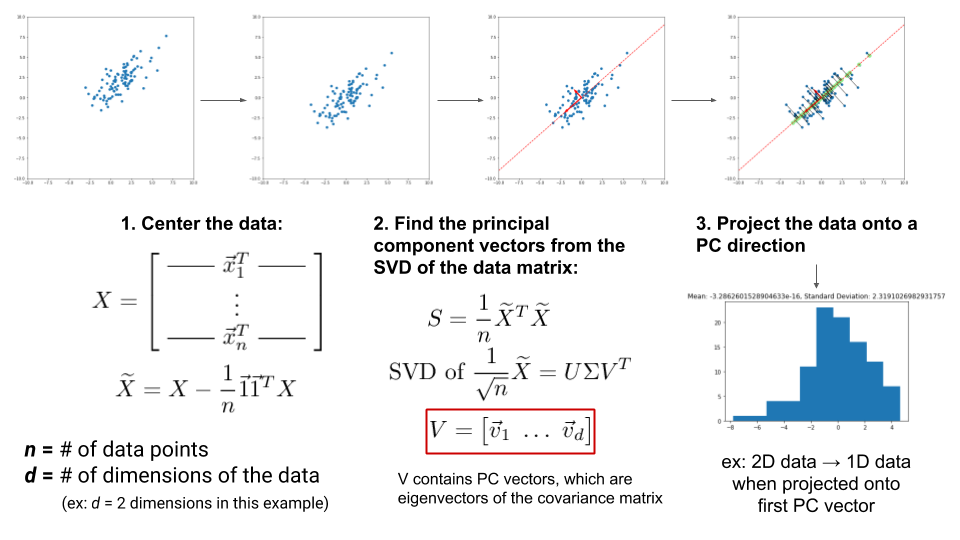
\includegraphics[width=\textwidth]{figures/pca-steps}

In summary,
\begin{enumerate}
    \item We first \textbf{demean} the data. If each datapoint is represented as a \textit{row}, then we are going to want to find the mean of each \textit{column} and subtract it from every element in that column to make it \textbf{zero-mean}. If each datapoint is a \textit{column}, we want every \textit{row} to be zero-mean.
    \item If each datapoint is a \textit{row} (as in the previous example), the covariance matrix is $\frac{1}{n} \widetilde{X}^T\widetilde{X}$, and the \textit{principal components} are the \textbf{columns of $V$} in the SVD (eigenvectors of the covariance matrix). 
    If each datapoint is a \textit{column}, the covariance matrix is $\frac{1}{n} \widetilde{X}\widetilde{X}^T$, and the \textit{principal components} correspond to the \textbf{columns of $U$}. \\
    \newline
    You can think of the covariance matrix as looking at the relation between the quantities we're measuring, and its eigenvectors as the directions in our data with the most variation.
    \item When you have the principal components, you can \textbf{project datapoints onto the principal components} to see how much of each principal component contributes to that datapoint.
\end{enumerate}

\newpage
\textbf{Minimum Norm Control} \\
Say we have a controllable system of rank $n$:
\begin{align*}
    \vec{x}(k + 1) = A\vec{x}(k) + \vec{b}u(k)
\end{align*}
 and we want to reach a desired state $\vec{x}_f$ with $k > n$ control inputs. We know we can reach any state in $n$ timesteps, and there are infinitely many ways to reach $\vec{x}_f$ in $k > n$ timesteps. Using the SVD however, we can find the series of control inputs that has the minimum norm. \\
 \newline
 Recall from the section on control that we can use the following linear system to solve for the control inputs:
 \begin{align*}
    \vec{x}(k) = \mathcal{C}_k \vec{u}_k
\end{align*}
\begin{align*}
    \vec{x}(k) = \begin{bmatrix}
        \vec{b} & A\vec{b} & \cdots & A^{k - 1} \vec{b}
    \end{bmatrix} \begin{bmatrix}
        u(k - 1) \\ \vdots \\ u(0)
    \end{bmatrix}
 \end{align*}

To solve for the minimum norm solution, we use the \textbf{Moore-Penrose Pseudoinverse}, a generalization of matrix inverses for rectangular matrices using the full SVD of a matrix. We denote the pseudoinverse with a dagger, and the solution will be $\vec{u}_k = \mathcal{C}_k^{\dagger} \vec{x}(k).$ 
This solution is special because it has \textbf{minimum norm}; that is, if we have another solution $\vec{z},$ such that $\mathcal{C}_k \vec{z} = \vec{x}(k),$ then $\norm{\vec{u}_k} \leq \norm{z}.$

To compute the pseudoinverse, we invert each element of the SVD one at a time:
\begin{align*}
    \mathcal{C}_k \vec{u}_k &= \vec{x}(k) \\
    U \Sigma V^T \vec{u}_k &= \vec{x}(k)\\
    (U^T U) \Sigma V^T \vec{u}_k &= U^T \vec{x}(k) \\
    (\Sigma^{\dagger} \Sigma) V^T \vec{u}_k &= \Sigma^{\dagger} U^T \vec{x}(k) \\
    (V V^T) \vec{u}_k &= V \Sigma^{\dagger} U^T \vec{x}(k) \\
    \vec{u}_k &= V \Sigma^{\dagger} U^T \vec{x}(k) \\
    \implies \vec{u}_k &= \mathcal{C}_k^{\dagger} \vec{x}(k)
\end{align*}

We can calculate $\Sigma^{\dagger}$ accordingly to produce an identity matrix such that the term $\Sigma^{\dagger}\Sigma$ disappears:

$$\Sigma^{\dagger} = \begin{bmatrix} \frac{1}{\sigma_{1}} & 0 &  \cdots & 0 \\ 0 & \frac{1}{\sigma_{2}} & \cdots & 0 \\ \vdots & \vdots & \ddots & \frac{1}{\sigma_{m}} \\ 
    \vdots & \vdots & \ddots & 0 \\ 0 & 0 & 0 & 0 \end{bmatrix}$$

\textit{Note}: This is another, sometimes computationally easier, form of the pseudoinverse:
$$\vec{u}_k = \mathcal{C}_k^T(\mathcal{C}_k\mathcal{C}_k^T)^{-1}\vec{x}(k)$$
See Sp20: Note 11B for more information.

\newpage

\subsection*{Signals}
\textbf{Sampling} \\
Although discrete-signals exist within the real world, many signals that we interact with are continuous. In order to do meaningful work processing them on a computer, we have to \textbf{discretize} the signal through the process of \textbf{sampling}.

\begin{figure}[H]
    \begin{tikzpicture}
        \node (left) {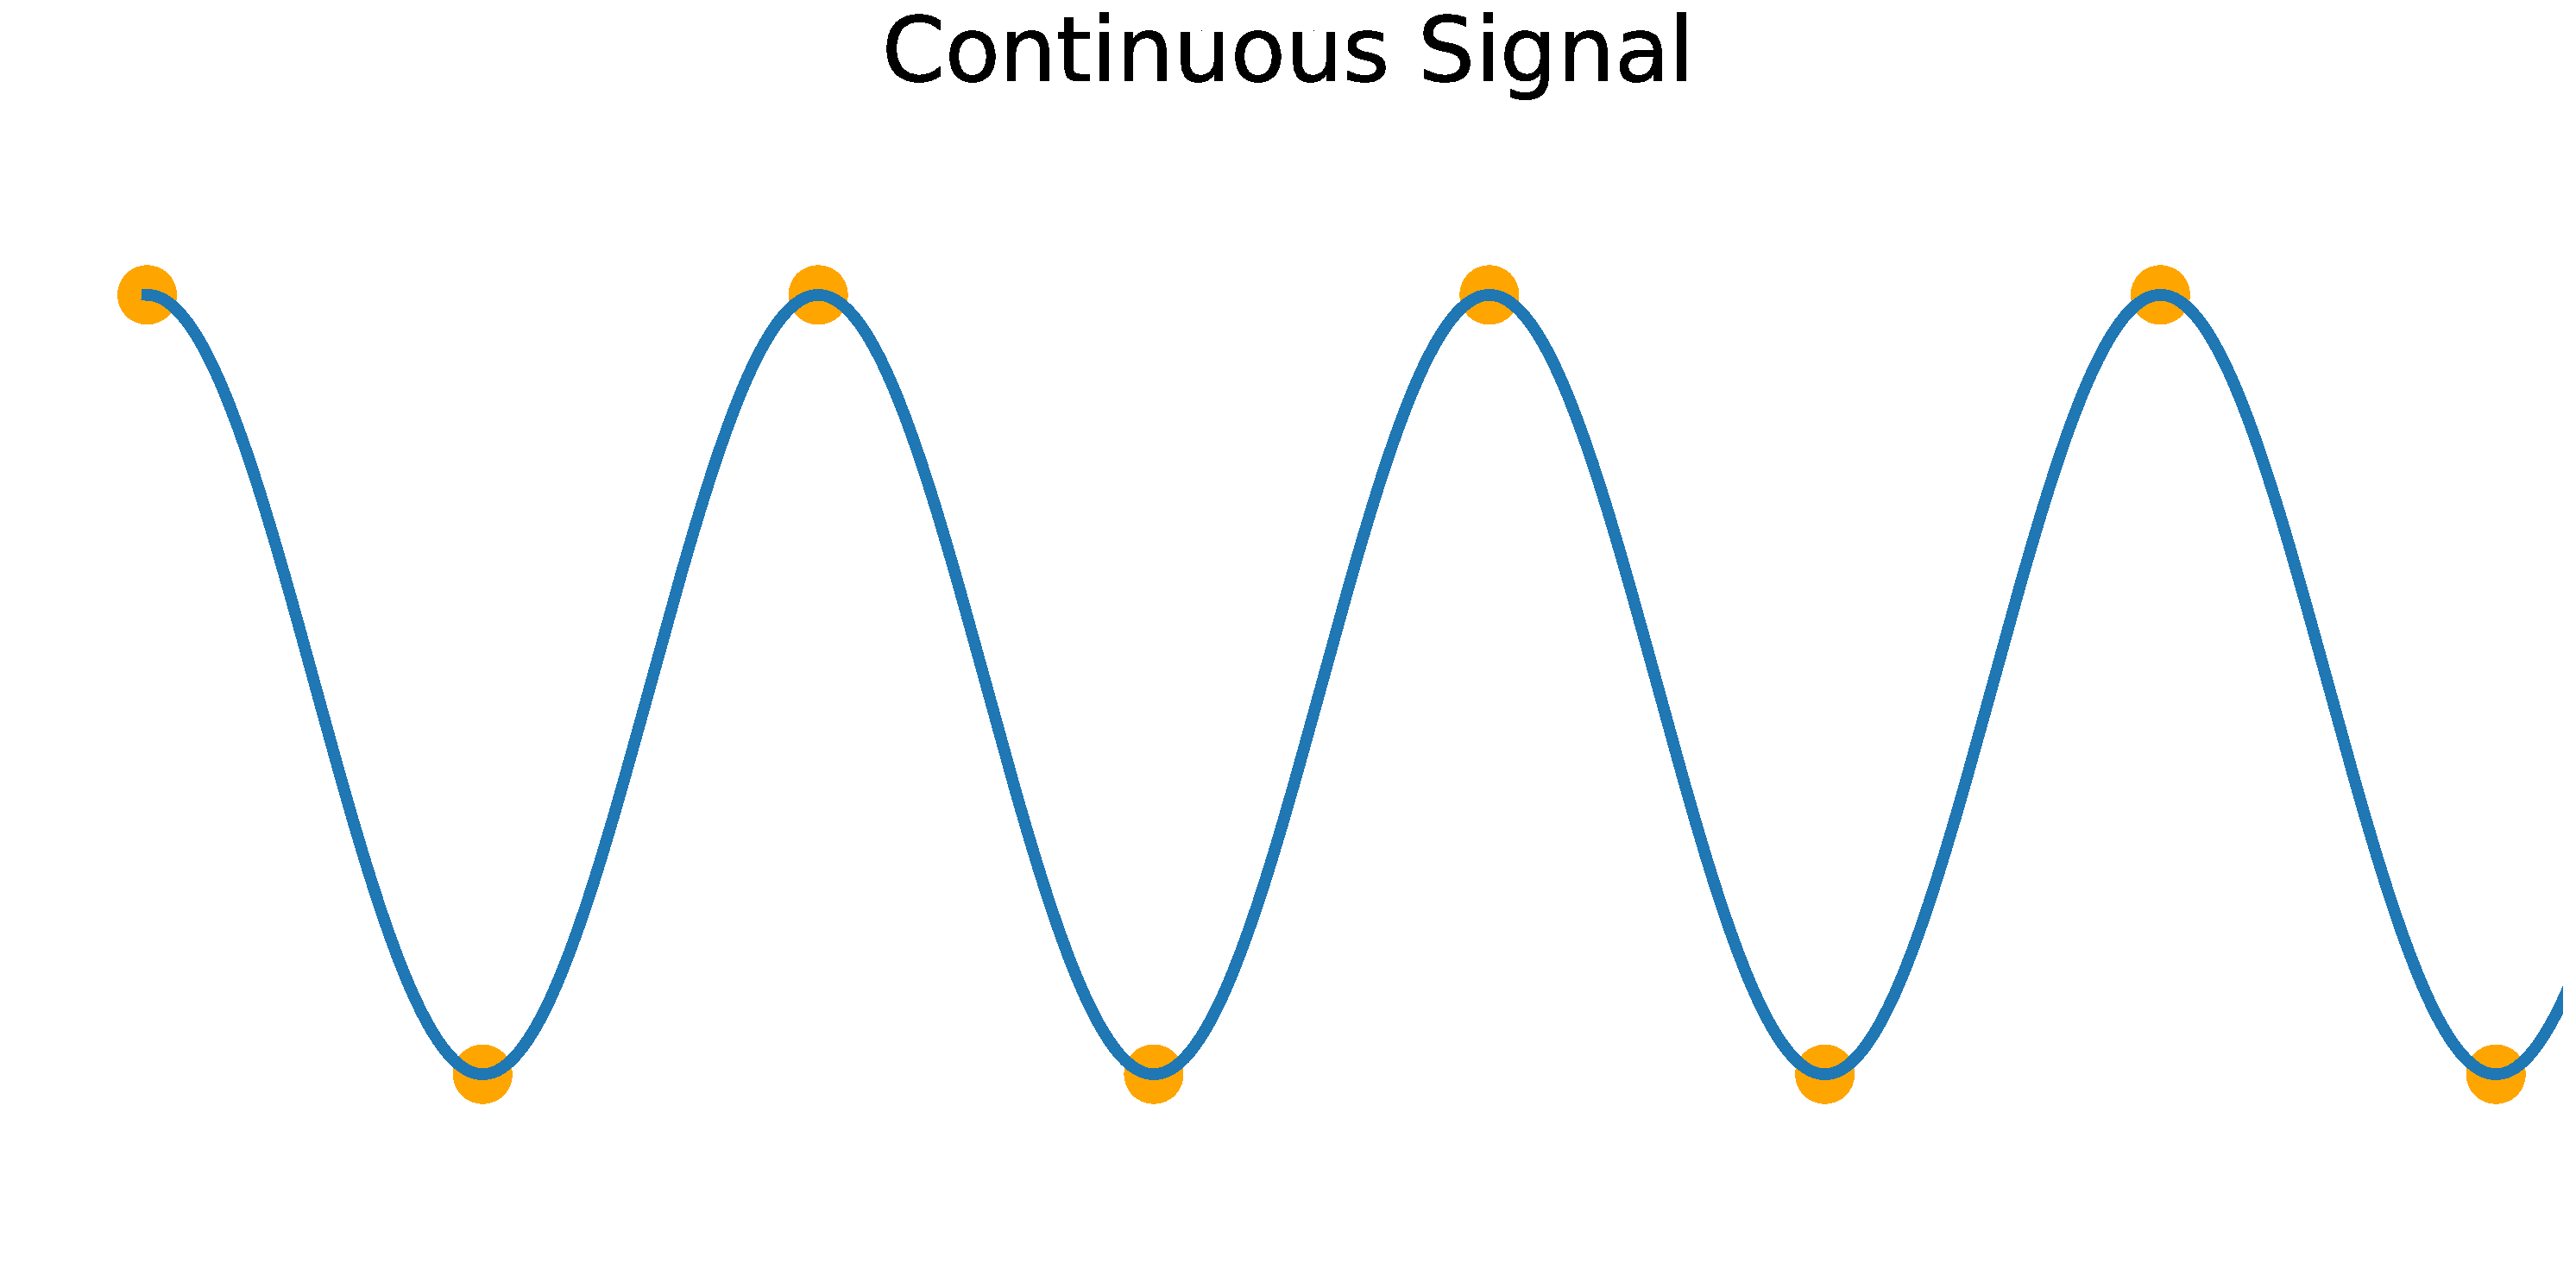
\includegraphics[width=8cm]{figures/continuous}};
        \node (right) [right=of left] {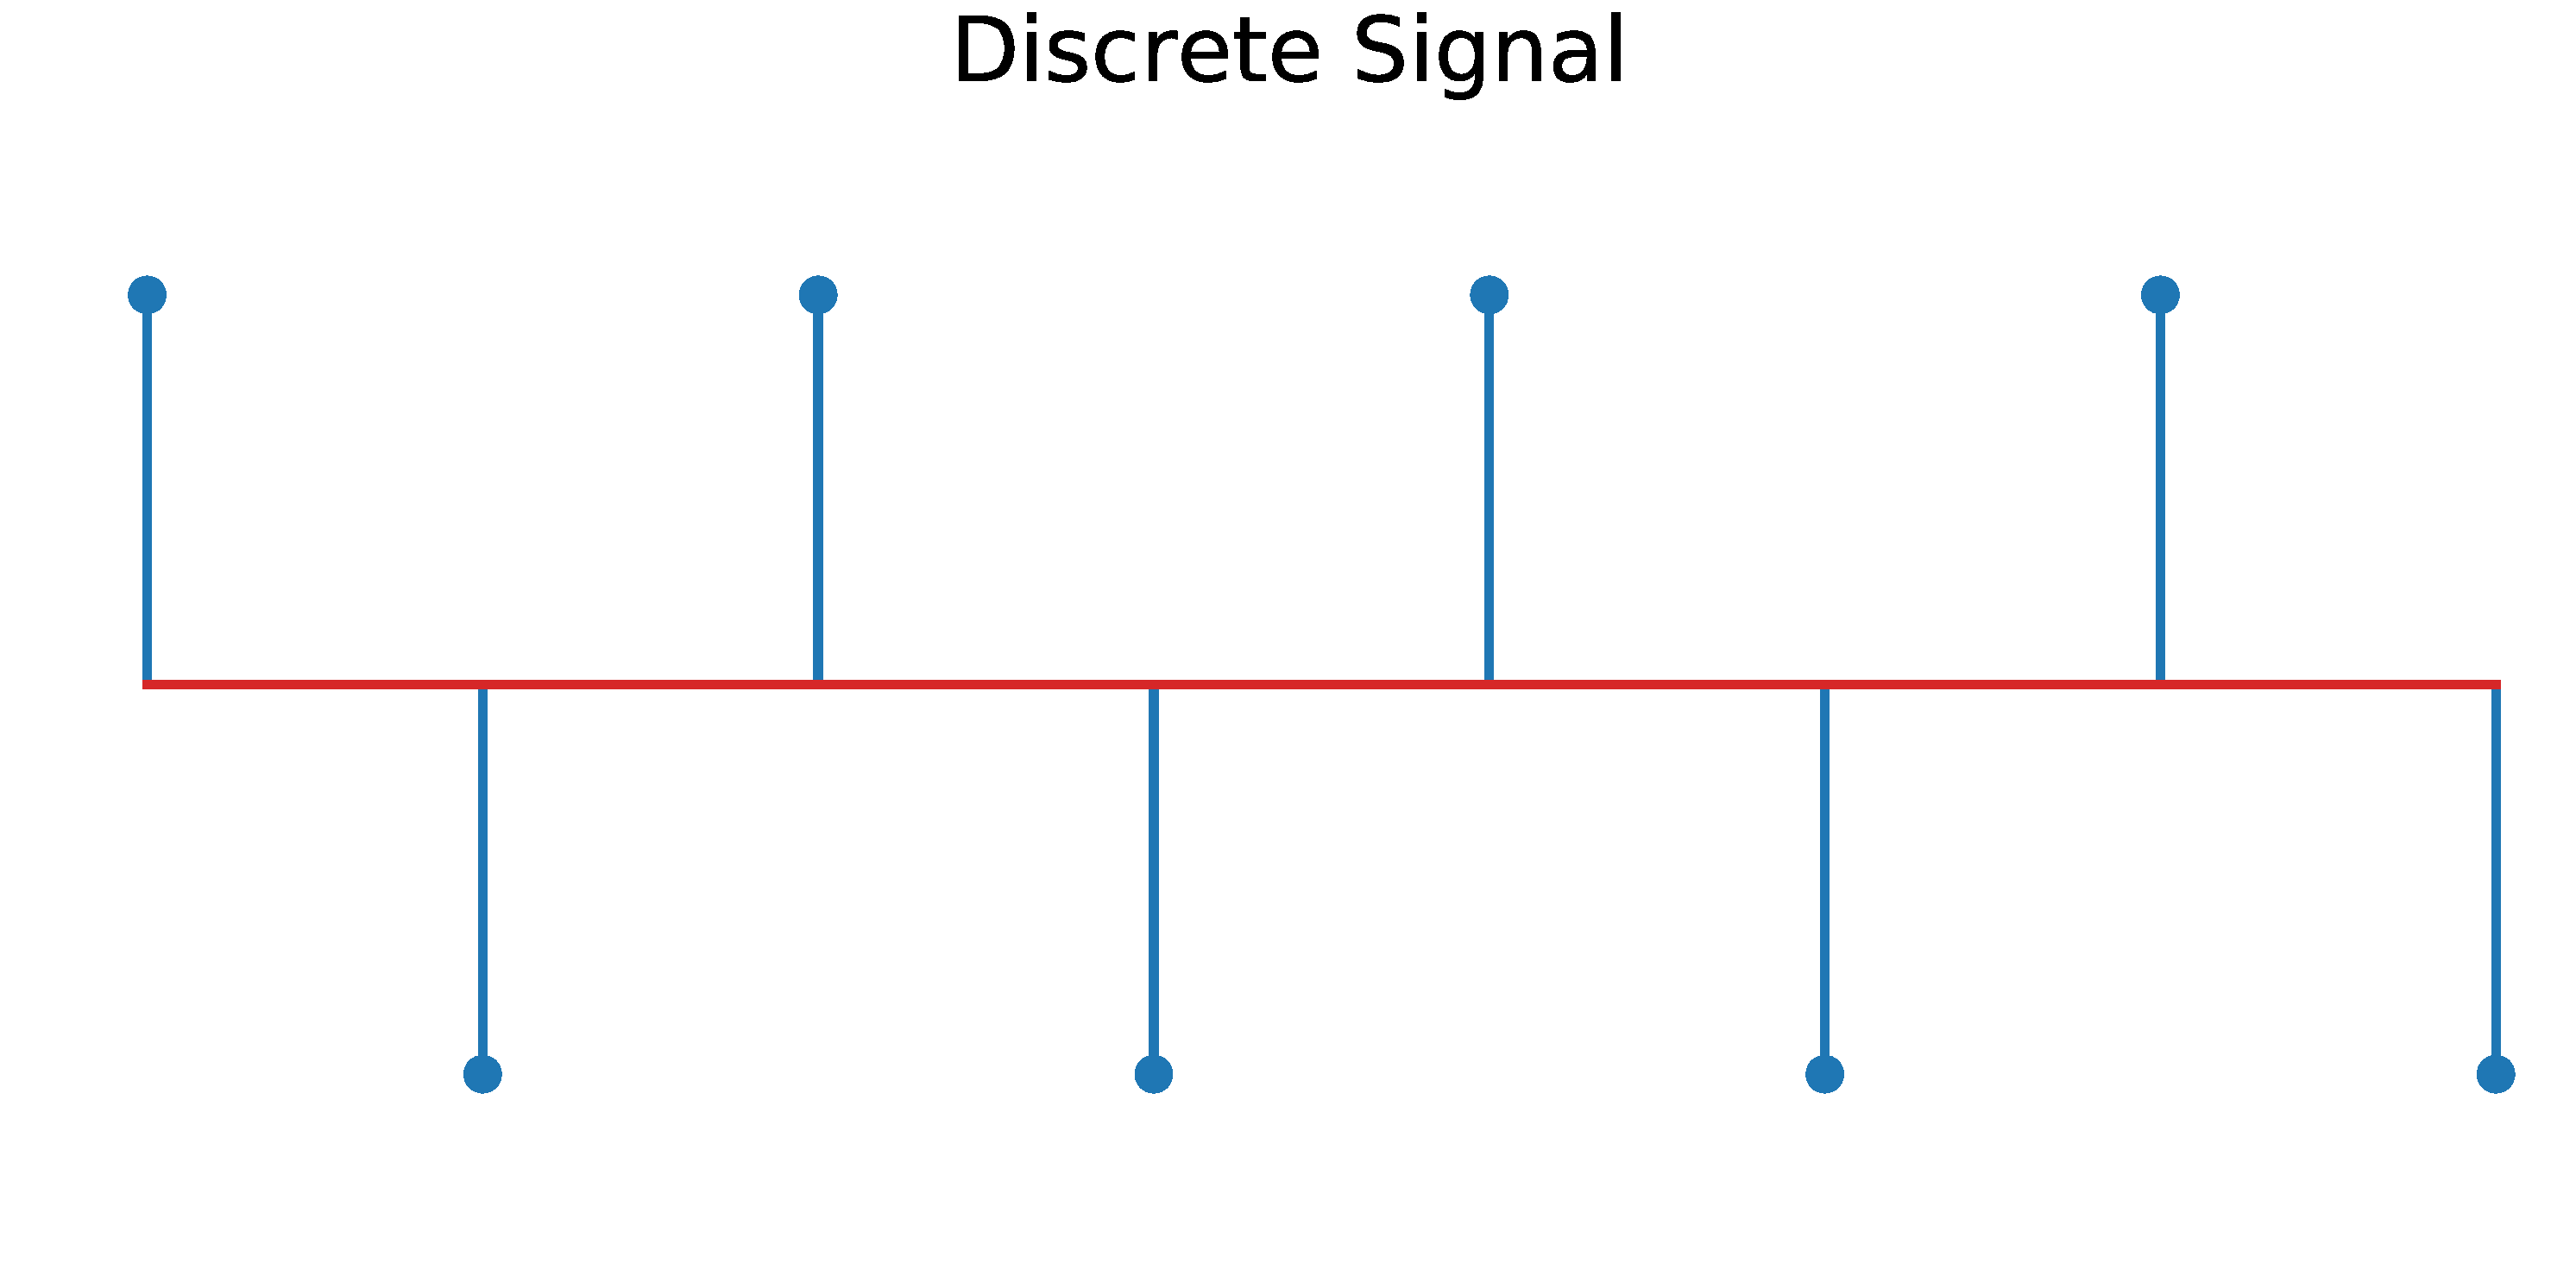
\includegraphics[width=8cm]{figures/discrete}};
        \path[->] [line width = .5mm] (left) edge (right);
    \end{tikzpicture}
\end{figure}

Sampling lets us turn a originally continuous-time signal into a discrete-time signal by taking points at evenly spaced intervals called the \textbf{sampling period} $\Delta$. We can also say that we take samples given by the \textbf{sampling frequency} $\frac{1}{\Delta}$. Properties of the original signal as well as the sampling frequency will determine how will we can reconstruct the signal from its samples later.

\textbf{Convolution} \\
With a discrete-time signal in our grasp, we will want to 

\textbf{Interpolation} \\
We saw that \textbf{sampling} lets us take a signal defined in continuous-time and convert it to a discrete-time representation.
The inverse problem to this is \textbf{interpolation}, which is all about going from a discrete-time representation of a signal $x[i]$ to the continuous-time representation $x(t)$.

\begin{figure}[H]
    \begin{tikzpicture}
        \node (left) {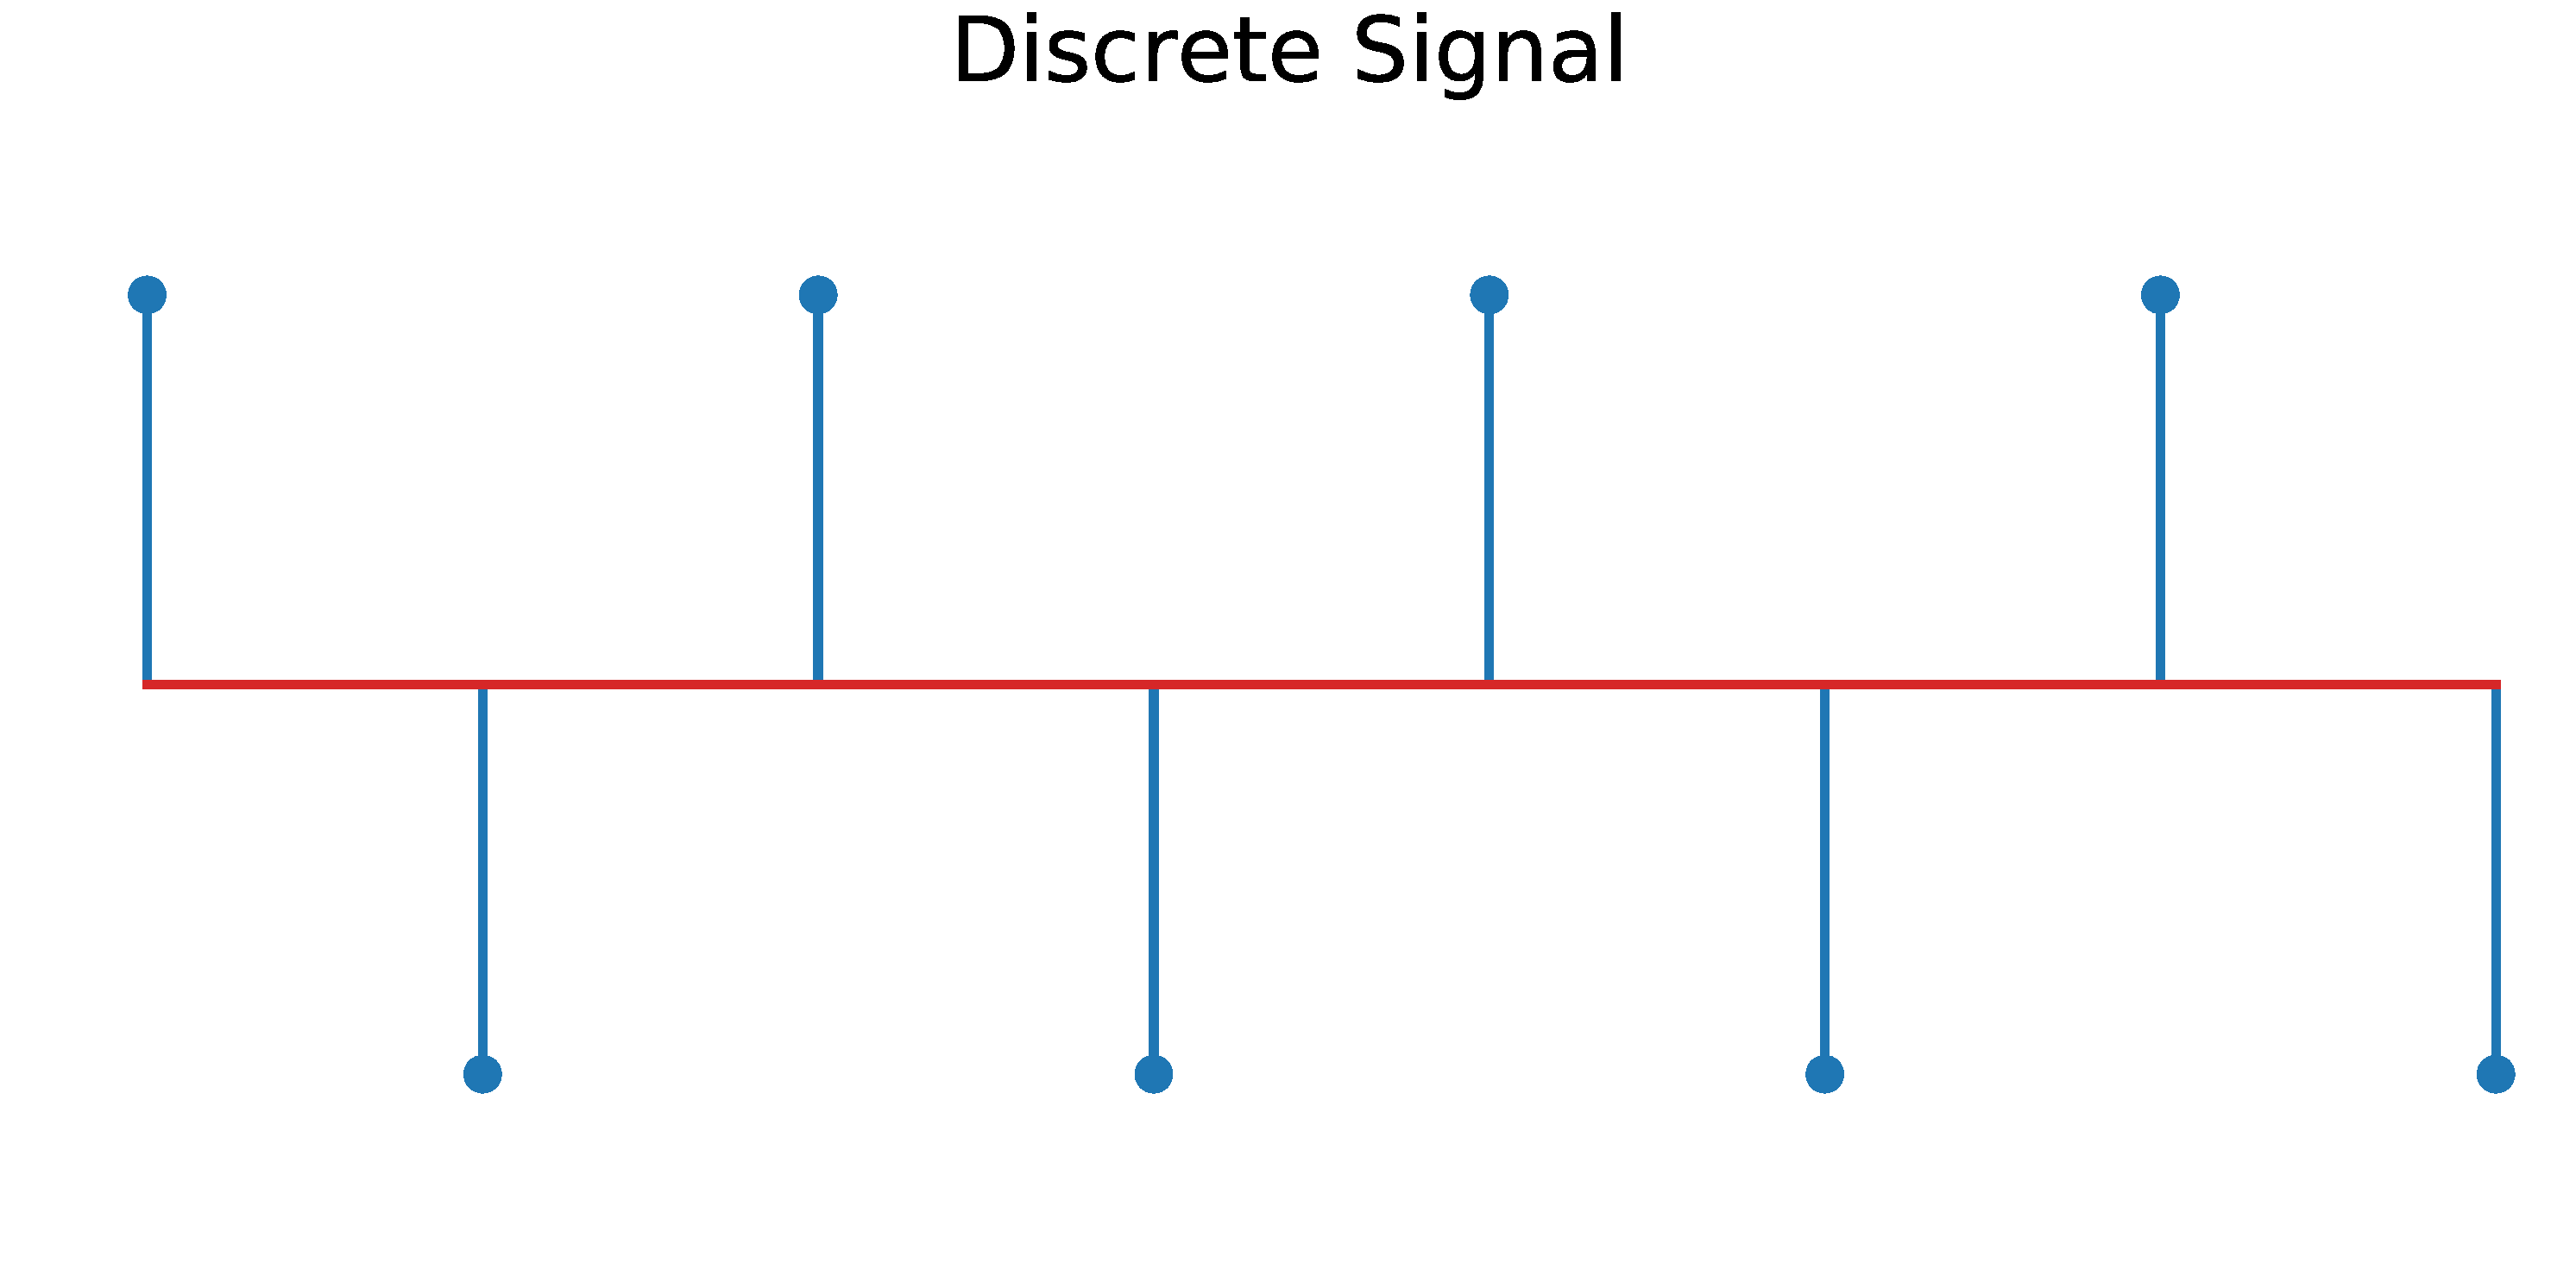
\includegraphics[width=8cm]{figures/discrete}};
        \node (right) [right=of left] {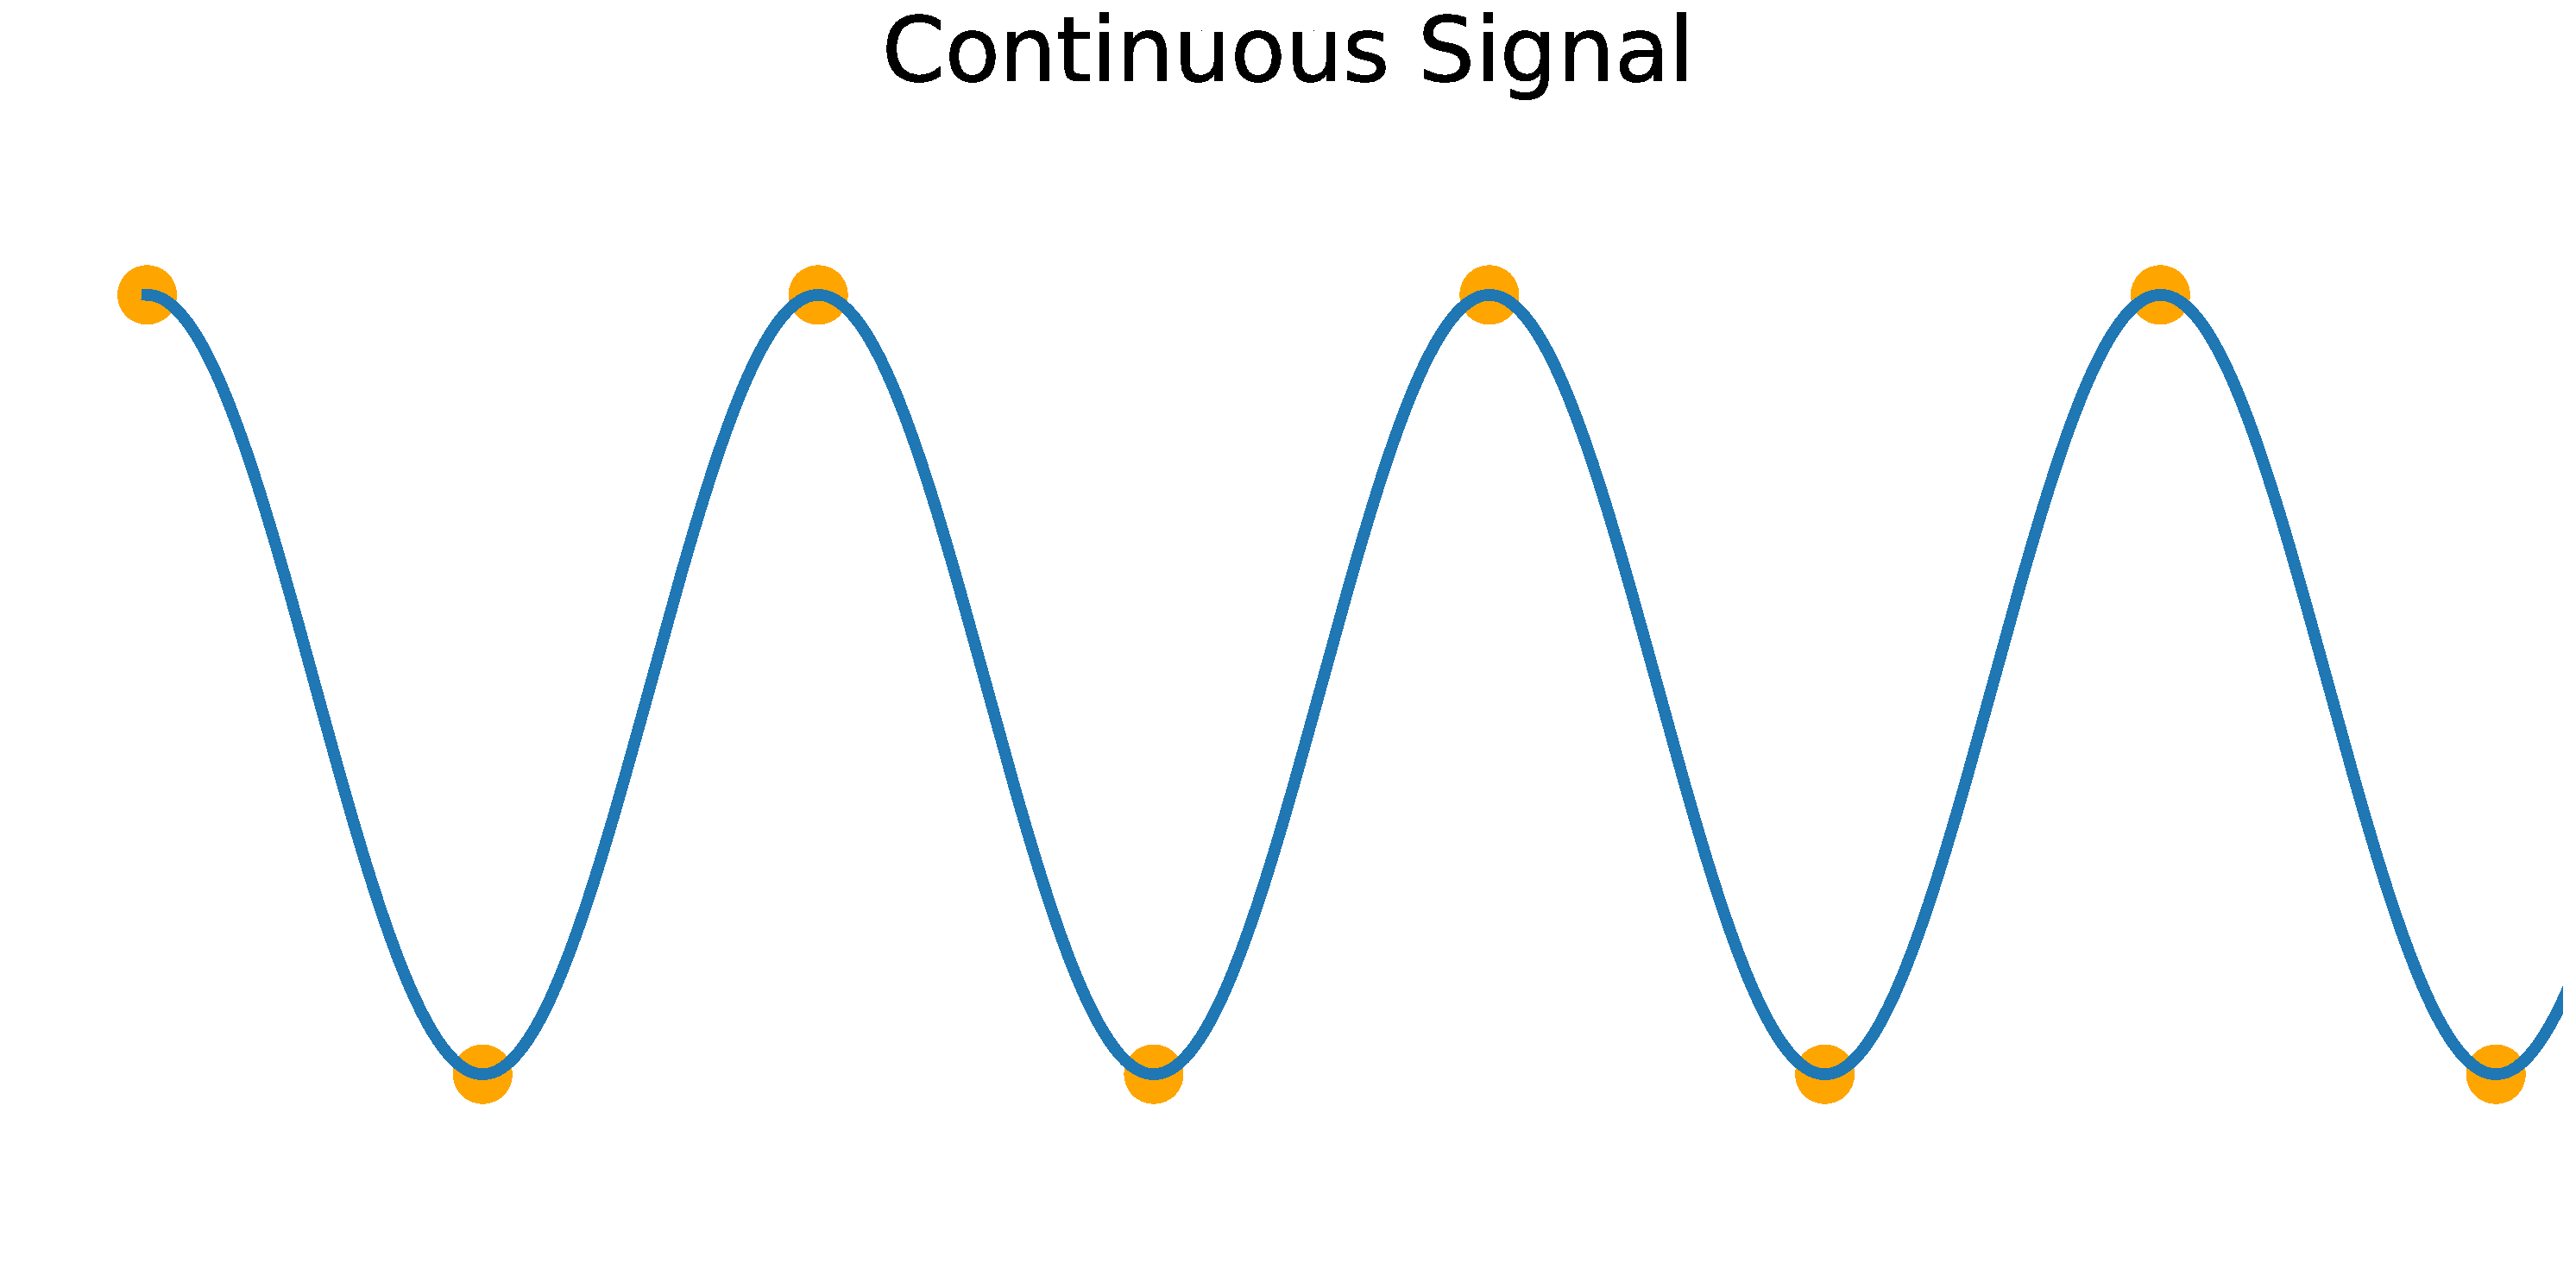
\includegraphics[width=8cm]{figures/continuous}};
        \path[->] [line width = .5mm] (left) edge (right);
    \end{tikzpicture}
\end{figure}

We may formalize the problem as follows: Given a discrete-time signal $x[i]$ with sampling period $\Delta$ (and therefore sampling frequency $\frac{1}{\Delta}$), we aim to generate a continuous-time signal $x(t)$ such that 

\begin{equation*}
\forall i \in \mathbb{Z}, x(i \Delta) = x[i]
\end{equation*}

In words, this means that our interpolated signal $x(t)$ must go through each sample from the discrete-time signal $x[i]$.
This is the main point which causes interpolation to differ from \textbf{regression}.
With regression, we also seek to extrapolate information from sampled data, however we don't seek to exactly fit the sampled data.
Instead, we aim to find the best approximation.
On the other hand, for a continuous-time signal to be a valid interpolation of a discrete-time signal, the continuous time signal \textbf{must} pass through each point specified by the discrete-time signal.
\newline
There are many ways to go about interpolation, but for 16B many of these ways all follow the same form.

\textbf{Basis Functions} \\
Recall that for a given vector space, we can form any vector in that vector space with a linear combination of a set of basis vectors.
Similarly, we are going to view interpolation through the lens of representing a continuous time signal as a linear combination of shifted basis functions, with weights determined by values of the of the discrete time signal.
\newline
For a basis function $\phi(t)$ to be valid, it must satisfy

\begin{equation*}
    \phi(0) = 1
\end{equation*}
and
\begin{equation*}
    \phi(k \Delta) = 0, k \in \mathbb{Z} \setminus 0
\end{equation*}

With these conditions satisfied, $\phi(t)$ produces the following interpolation: 

\begin{equation*}
    x(t) = \sum_{k=-\infty}^{k=\infty} x[k] \phi(t - k \Delta)
\end{equation*}

Essentially, for every sample in our discrete-time signal, we shift our basis function to that sample, scale by the value of the sample, and and add together all these shifted and scaled basis functions to produce our interpolation. The previously established conditions on $\phi(t)$ ensure that this shifting, scaling, and adding results in a valid interpolation, which we prove by confirming $x(i \Delta) = x[i]$.
\begin{equation*}
    x(i \Delta) = \sum_{k=-\infty}^{k=\infty} x[k] \phi(i \Delta - k \Delta
\end{equation*}
Using the defined properties of our basis function $\phi(t)$, we can simplify the summation.
\begin{align*}
\phi(i \Delta - k \Delta)
    &=
    \begin{cases}
        1 & i = k \\
        0 & \text{otherwise} \\
    \end{cases} \\
\sum_{k=-\infty}^{k=\infty} x[k] \phi(i \Delta - k \Delta) &= x[i] \\
x(i \Delta) &= x[i]
\end{align*}

Therefore, basis functions give us a valid interpolation. We will see different ways we can define our basis funtion to get many different interpolations, each with their own strenghts and drawbacks.

\textbf{Zero-Order Hold Interpolation} \\
The zero-order hold is the the interpolation we get when we hold the value of each sample in our discrete-time signal constant over the sampling interval.


\begin{figure}[H]
\centering
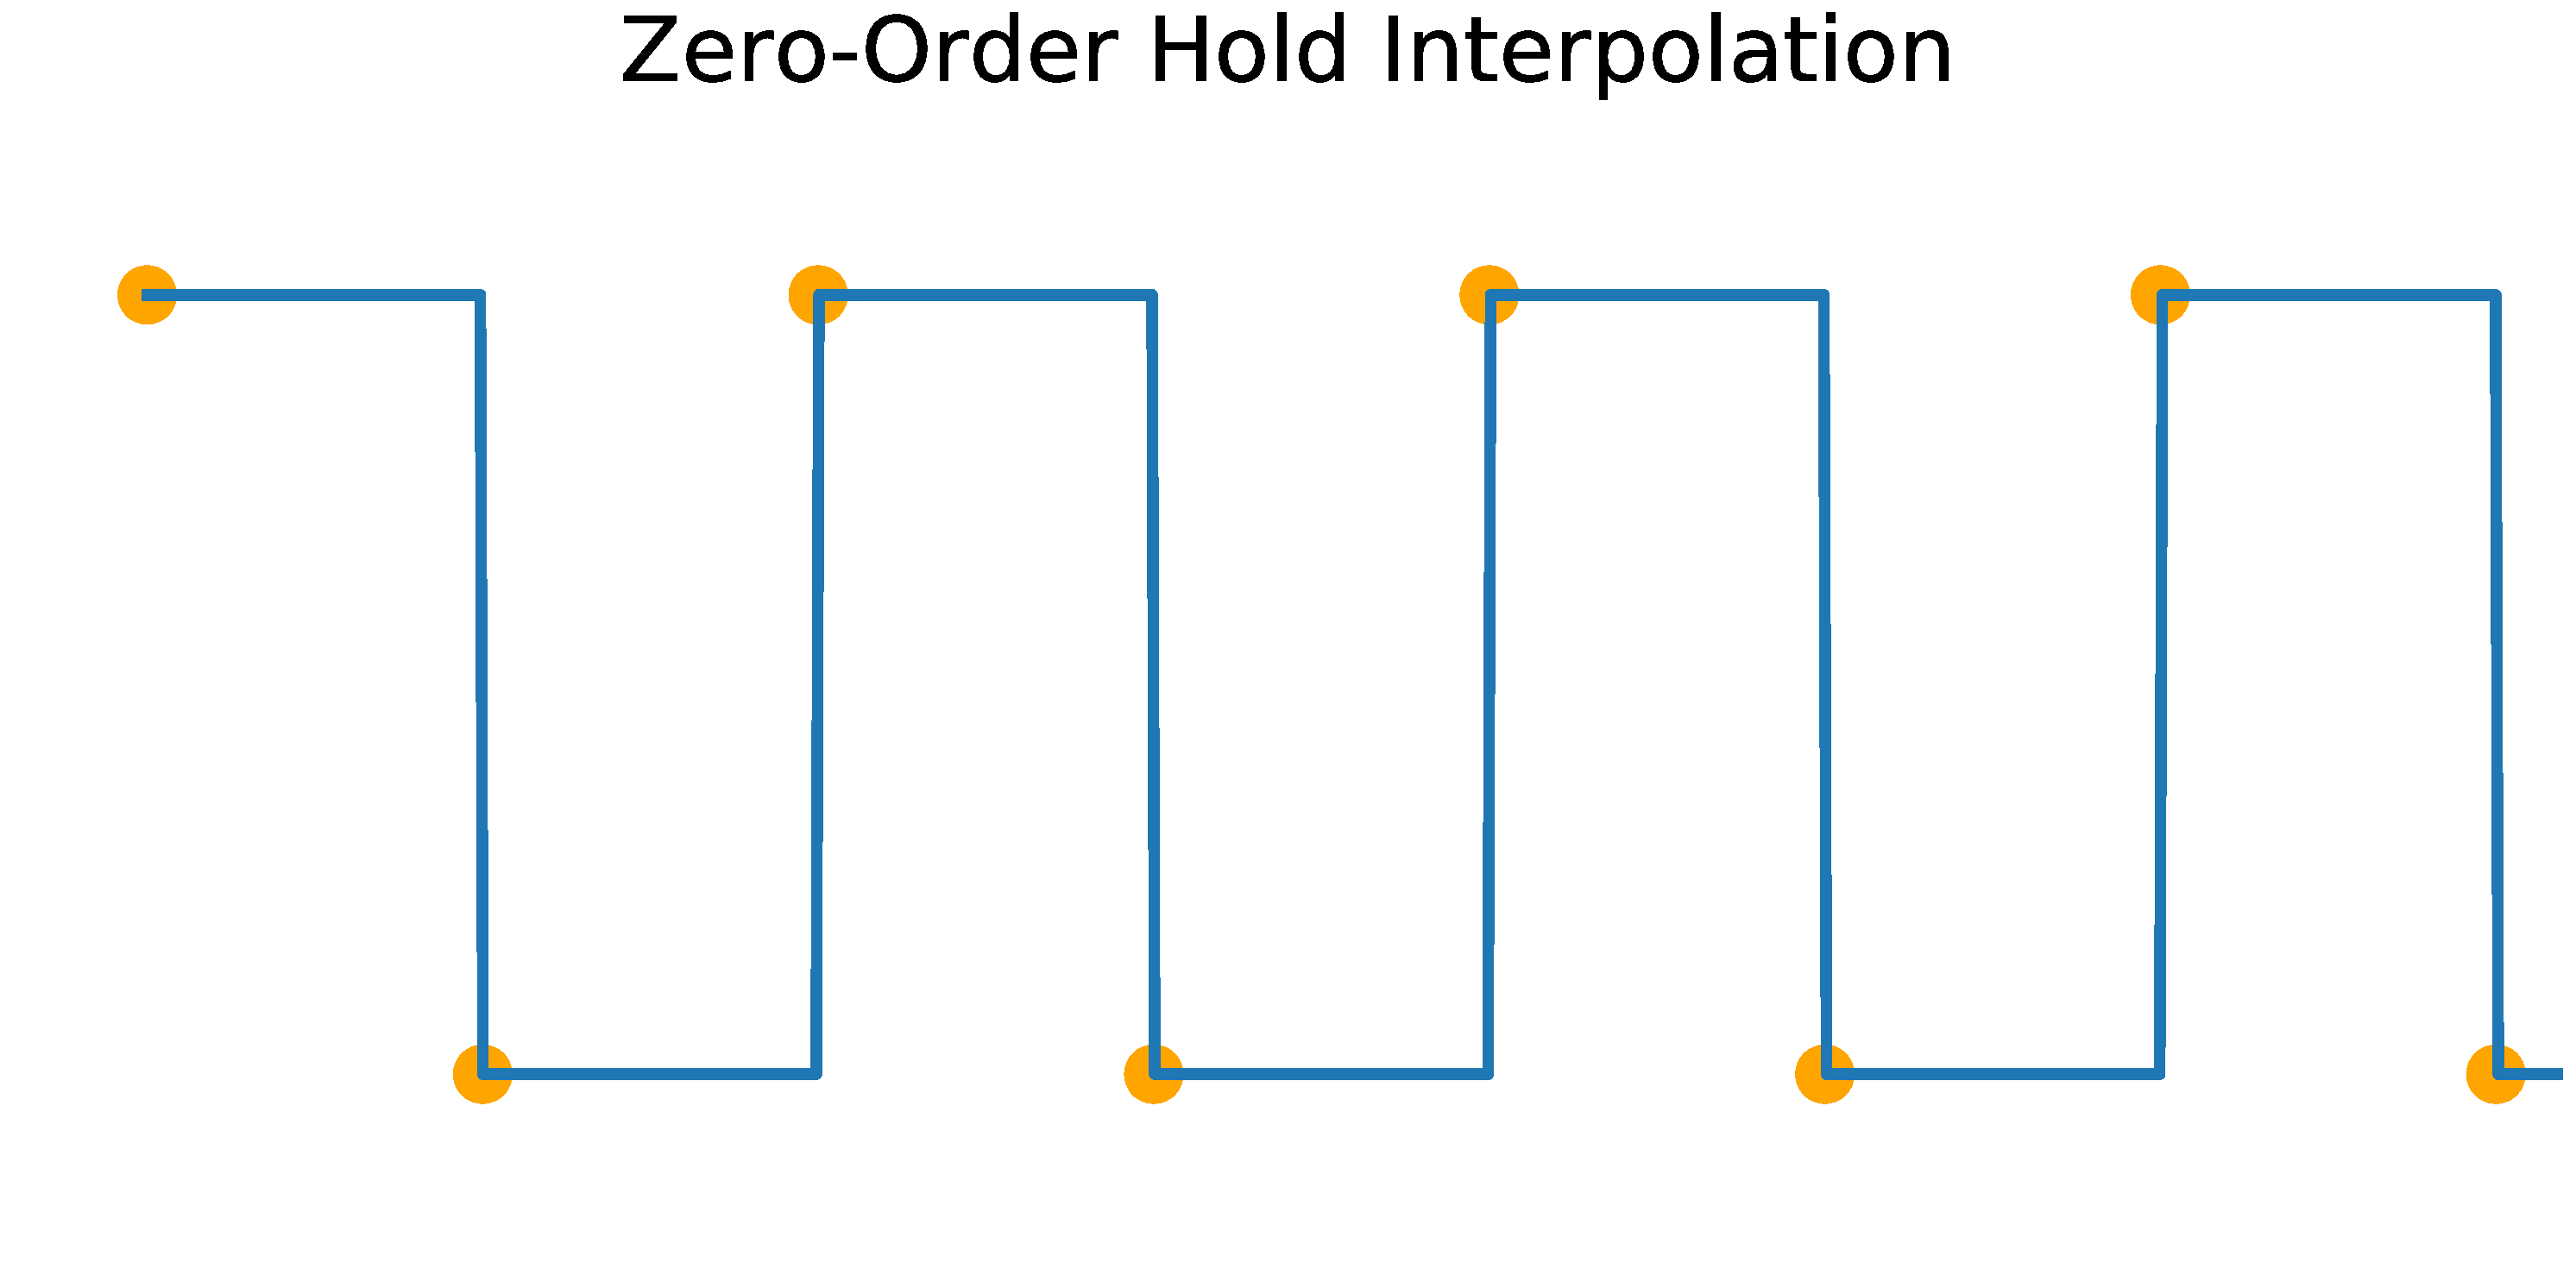
\includegraphics[width=.8\textwidth]{figures/zoh_interp}
\end{figure}

Formally, we may define the interpolation as
\begin{equation*}
    \forall i \in \mathbb{Z}, x(t) = x[i],\;t \in [i \Delta, (i + 1) \Delta
\end{equation*}

We can also define this interpolation using the basis function formulation.
\begin{equation*}
    \phi(t) = 
    \begin{cases}
    1 & t \in [0, \Delta) \\
    0 & \text{otherwise} \\
    \end{cases}
\end{equation*}


\begin{figure}[H]
\centering
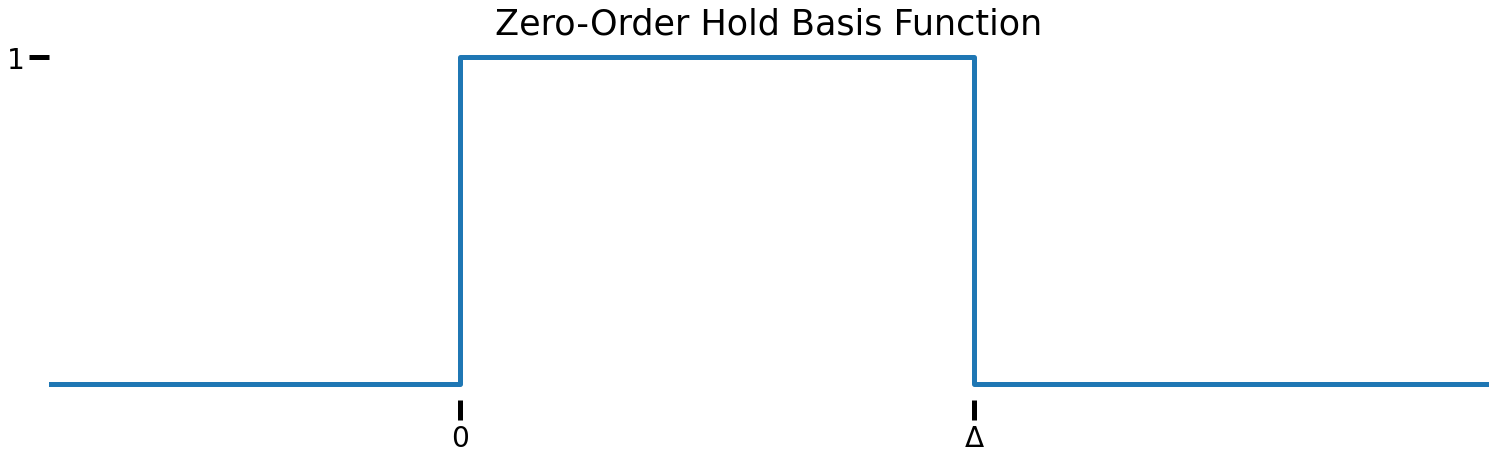
\includegraphics[width=10cm]{figures/zoh_basis}
\end{figure}


We saw that the zero-order hold assumes that our signal stayed constant between sample points. We know this is usually not the case. The following interpolations reconstruct a signal that can still have a change in value between sample points, which can produce a more accurate representation of the original signal.

\textbf{Linear Interpolation} \\
We can generate the linear interpolation of our signal by drawing straight lines between each of our samples.
Mathematically, this we define the reconstructed signal as
\begin{align*}
    x(t) &= x[i] + \frac{x[i + 1] - x[i]}{\Delta} \cdot (t - i \cdot \Delta) \\
    &= x[i] \cdot (1 - \frac{t - i \Delta}{\Delta}) + x[i + 1] \cdot (\frac{t - i \Delta}{\Delta}),\;t \in [i \Delta, (i + 1) \Delta)
\end{align*}
which we can derive by trying to fit a line between any two samples of the signal.
\newline
We also have a basis function we can use for linear interpolation.
\begin{equation*}
    \phi(t) = 
\begin{cases}
1 - \frac{\lvert t \rvert}{\Delta} & t \in [- \Delta, \Delta] \\
0 & \text{otherwise}
\end{cases}
\end{equation*}

\begin{figure}[H]
\centering
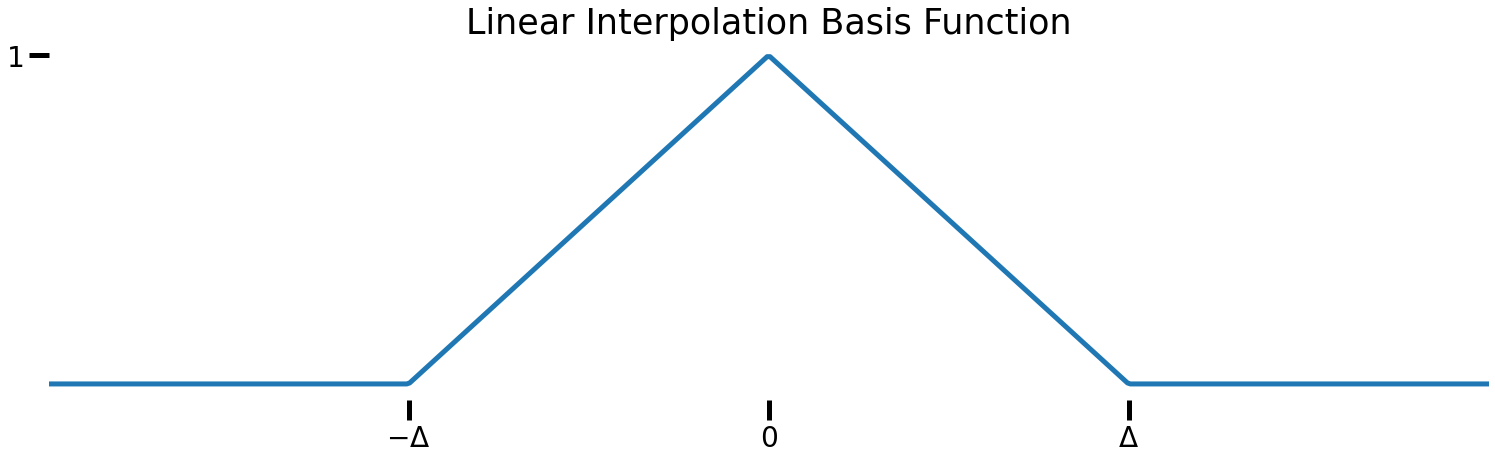
\includegraphics[width=.5\textwidth]{figures/lin_basis}
\end{figure}

We can apply the basis function for interpolation as shown below.
\begin{figure}[H]
    \begin{tikzpicture}
        \node (left) {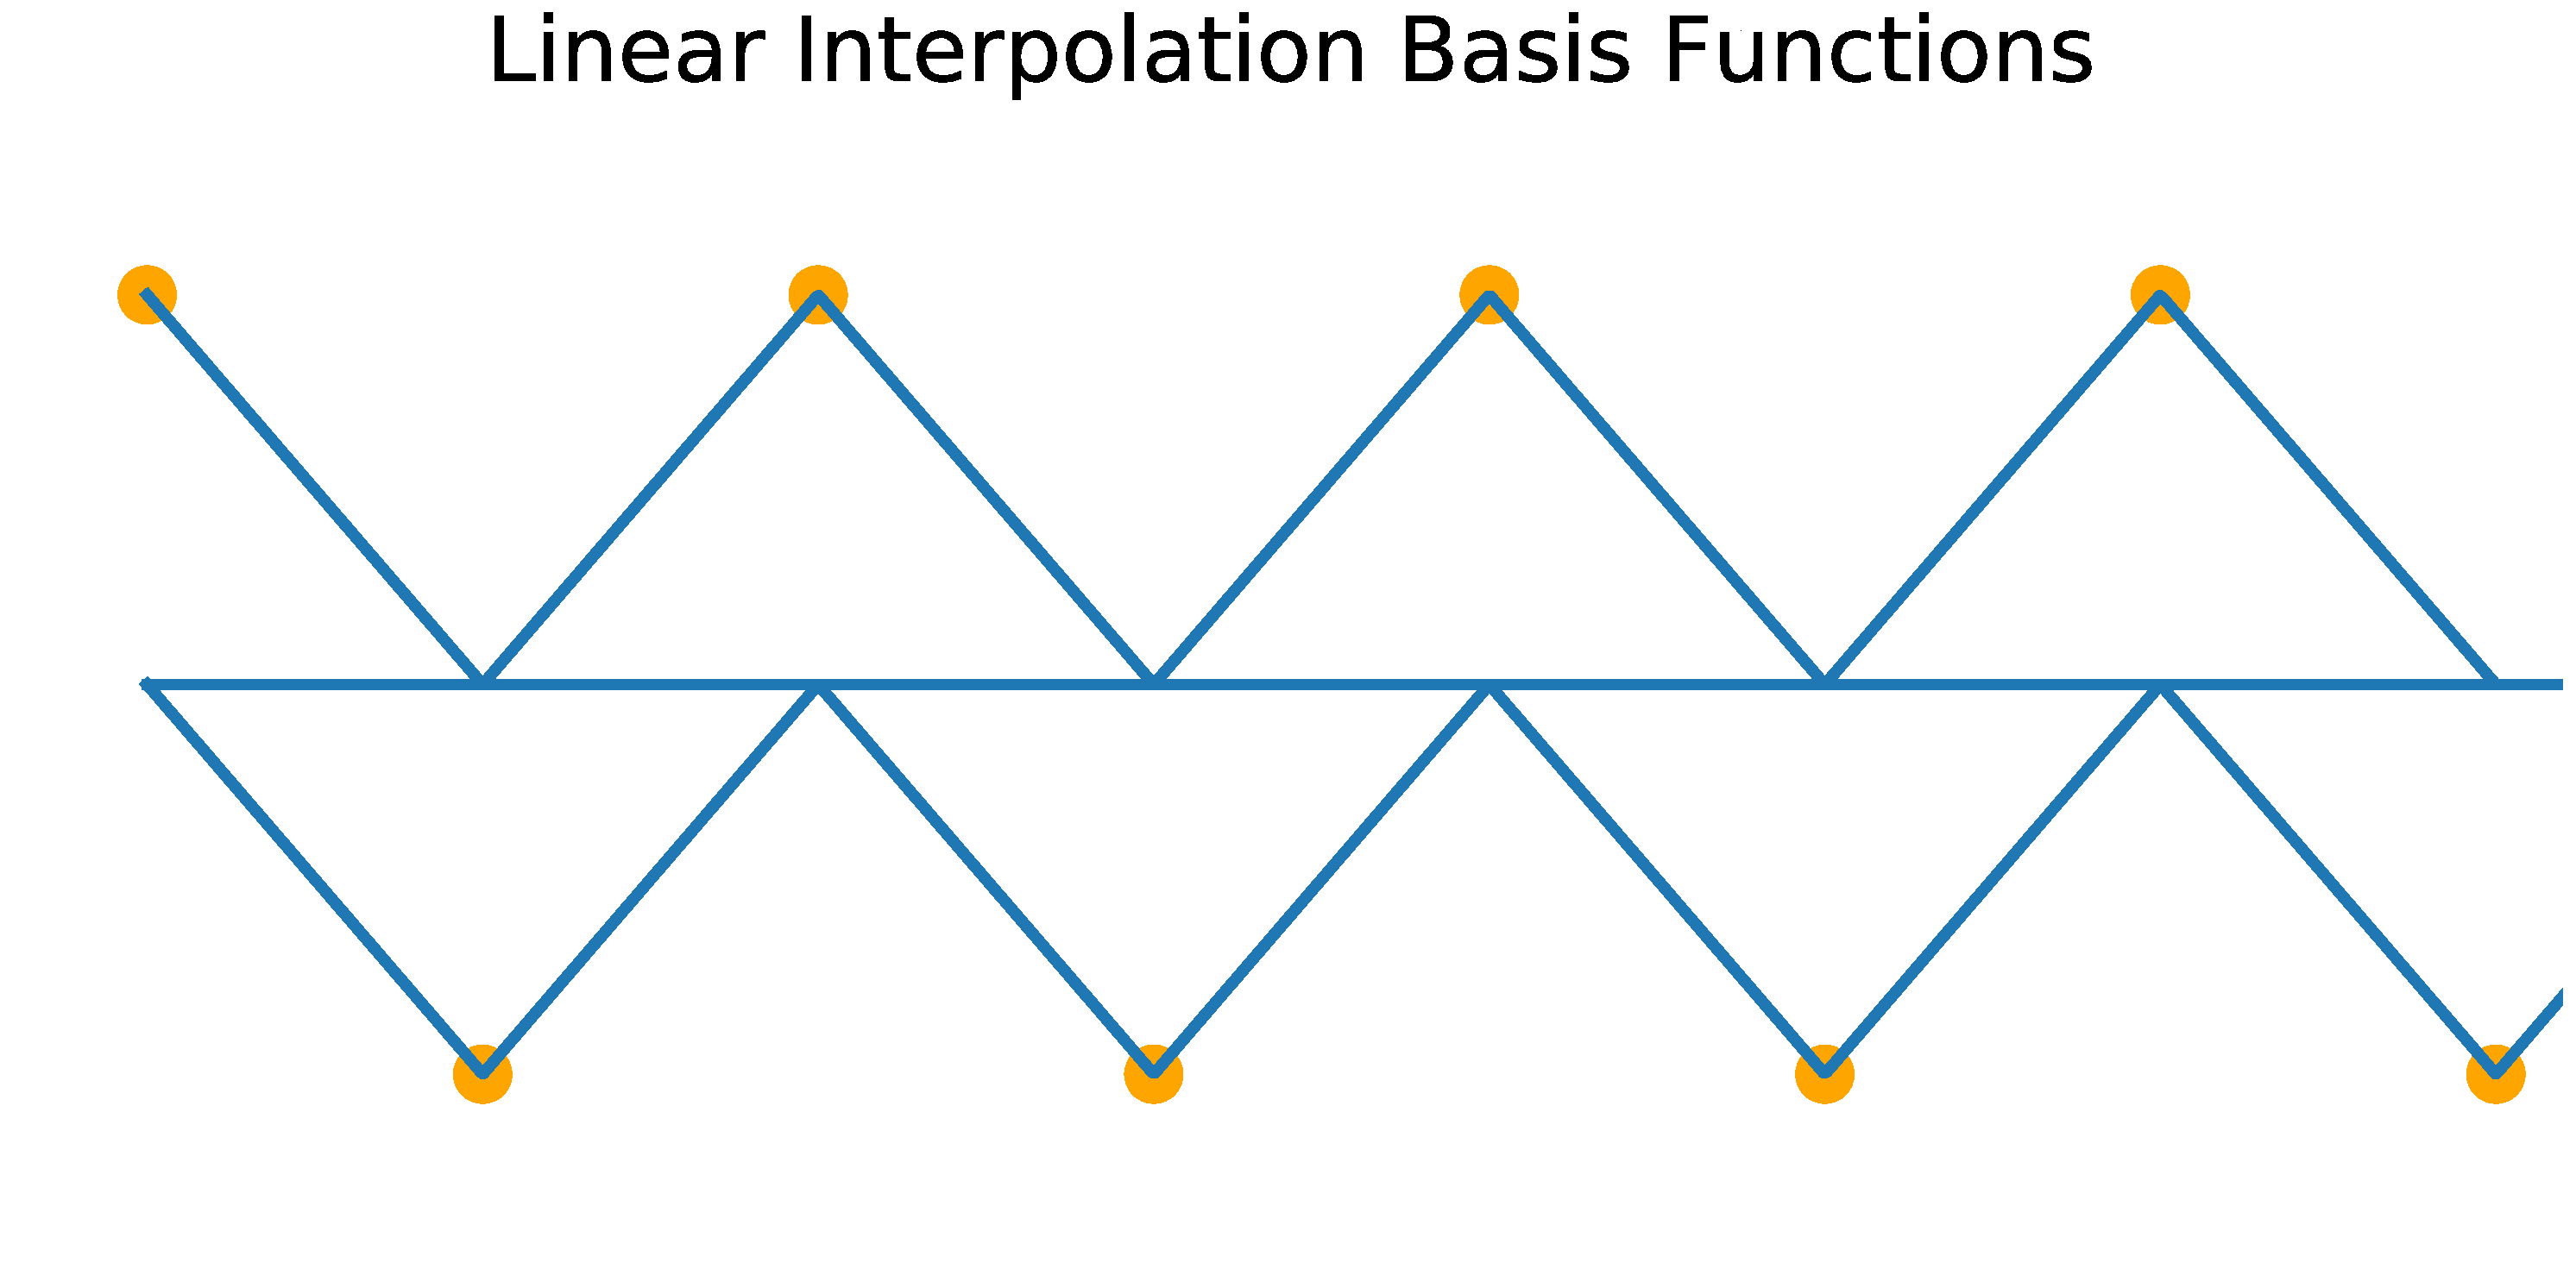
\includegraphics[width=8cm]{figures/lin_basis_interp}};
        \node (right) [right=of left] {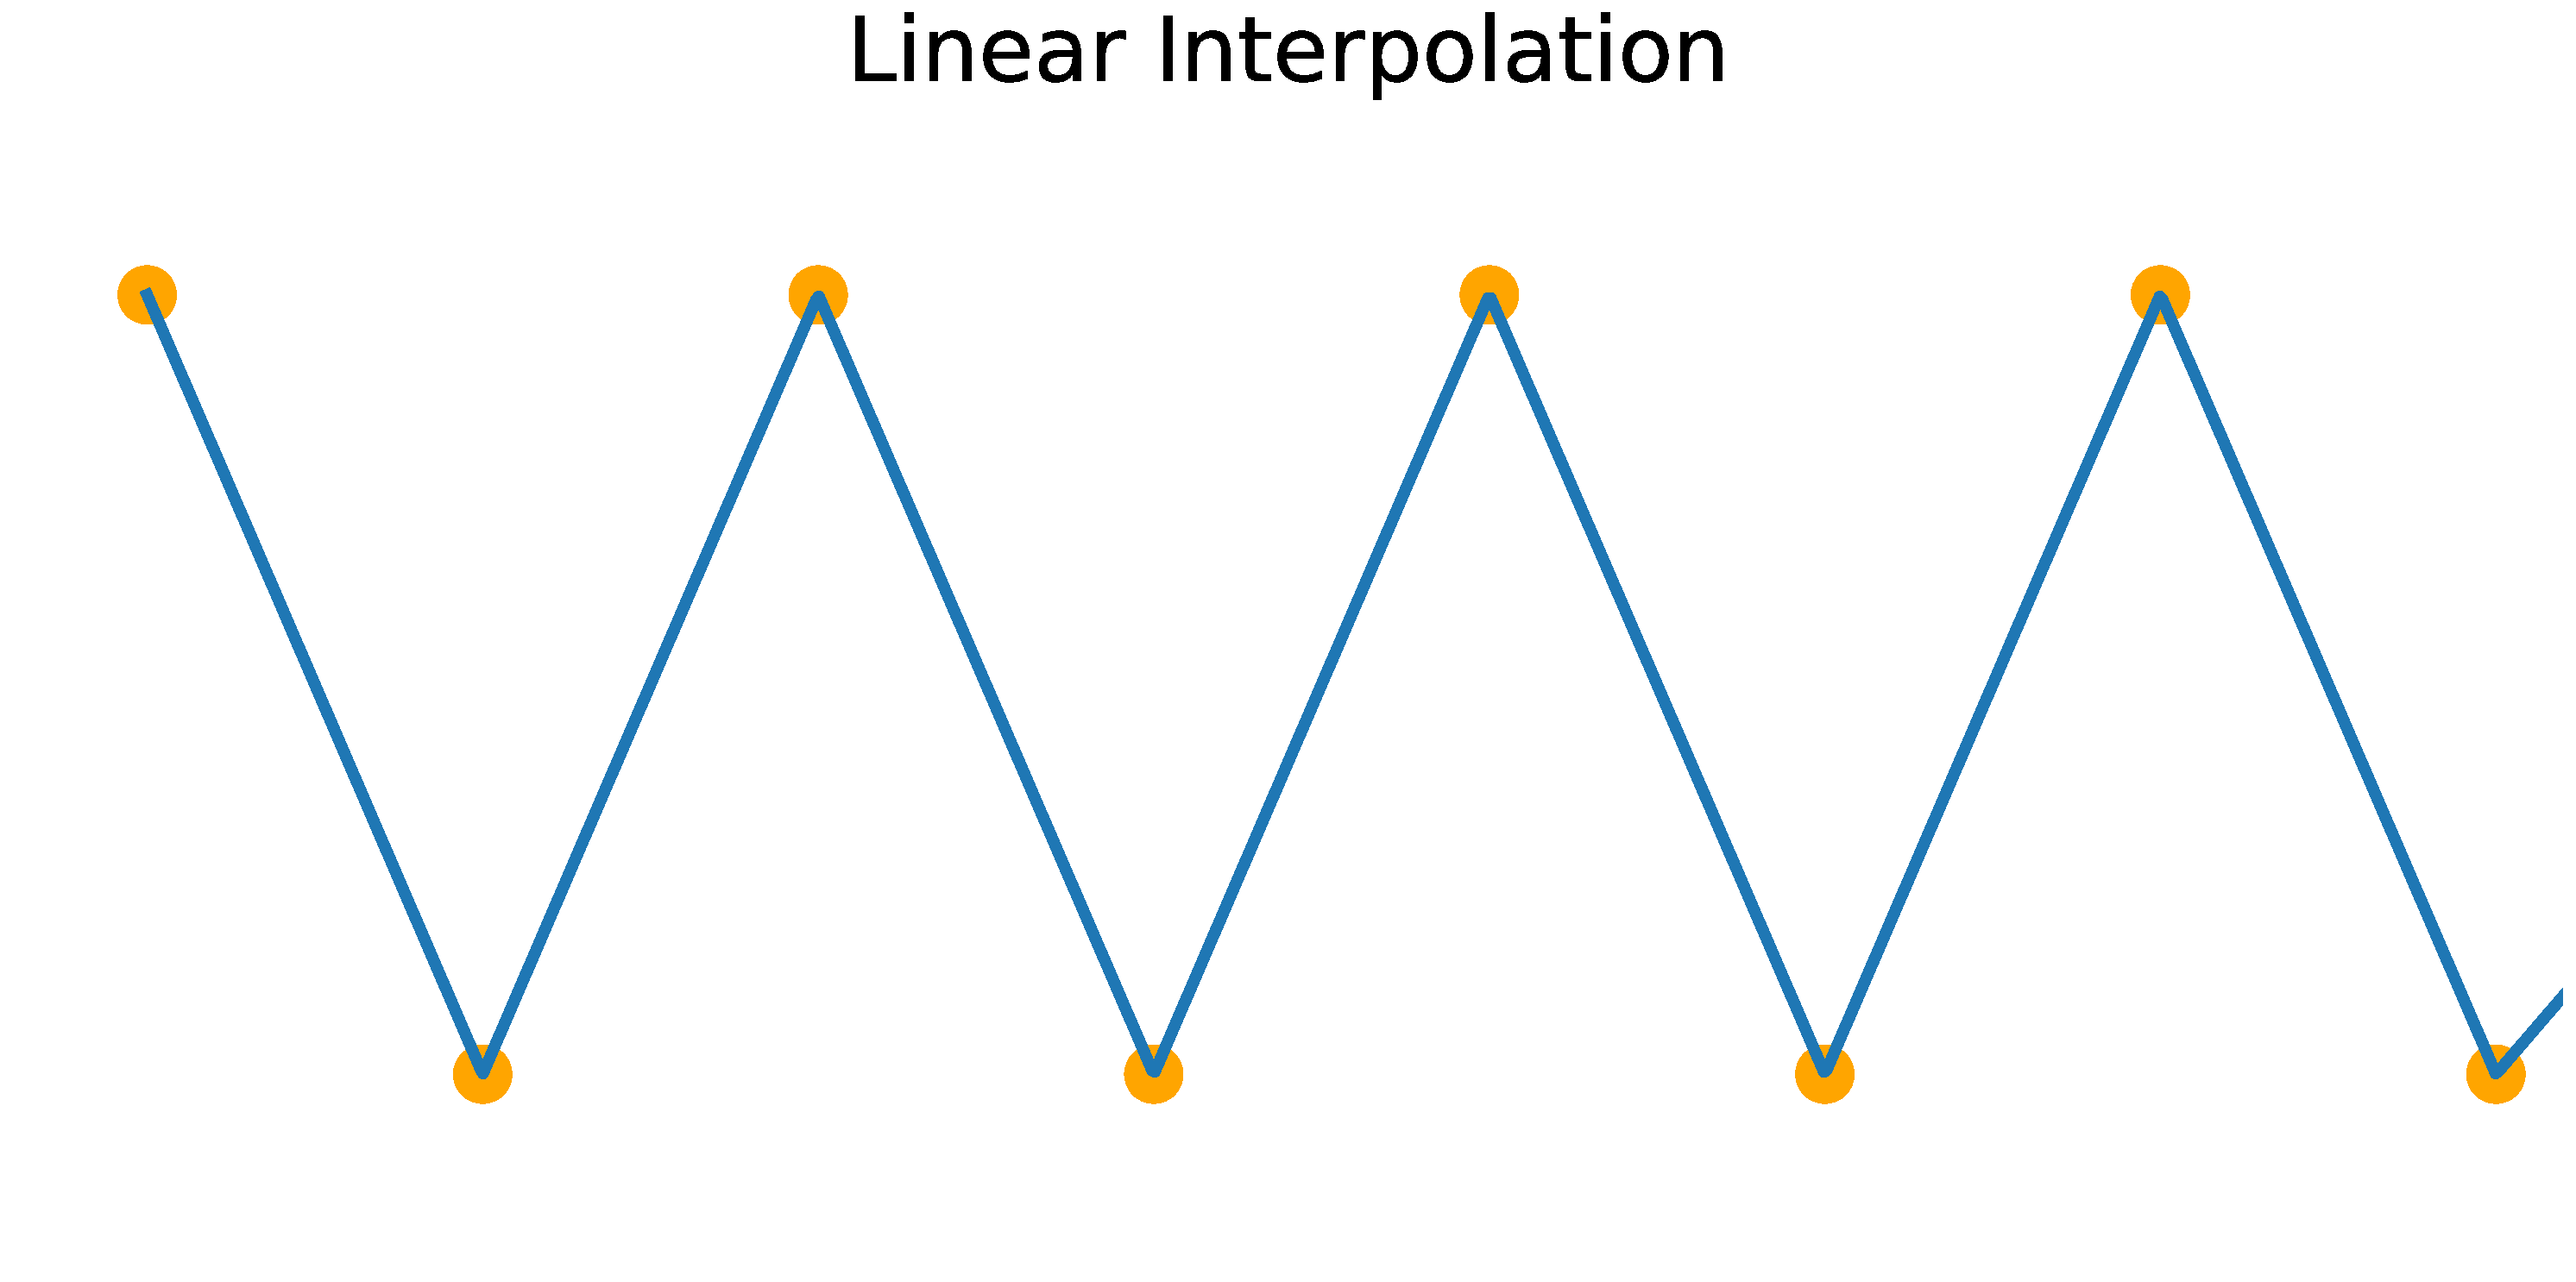
\includegraphics[width=8cm]{figures/lin_interp}};
        \path[->] [line width = .5mm] (left) edge (right);
    \end{tikzpicture}
\end{figure}
Since each basis function creates a line that starts at a sample point and goes to $0$ at adjacent sample point, summing up all these lines ensures that there is line going between each sample point.

\textbf{Polynomial Interpolation} \\
While the zero-order hold and linear interpolation cannot really reconstruct any smoothness in our original signal, we will see that polynomial interoplation is very capable of such a feet. Recall that $n$ points uniquely definine a polynomial of degree $\leq n - 1$ (ex. 2 points can define exactly one straight line going through them, but an infinite number of quadratic functions. 3 points will uniqueuely define a quadratic, we still have an infinite number of cubics, and so on \ldots). Thus, if we have collected a $n$ samples of our siginal that we wish to interpolate with, we will try to fit a polynomial of degree at most $n-1$ through those points. Such a polynomial has general form
\begin{equation*}
    x(t) = a_0 + a_1 t + \dots + a_{n-1} t^{n-1} 
\end{equation*}
The free parameters of our interpolation are the variables coefficients $a_0, a_1, \ldots, a_{n-1}$. We just need to choose the coefficients such that we satisfy the only constraint of our interpolation.
\begin{equation*}
    x(i \Delta) = x[i]
\end{equation*}
This property lets us setup a system of equations
\begin{align*}
x(i_1 \Delta) &= x[i_1] \\
x(i_2 \Delta) &= x[i_2] \\
\vdots \\
x(i_n \Delta) &= x[i_n] \\
\end{align*}
where $i_k$ represents the index of the $k\textsuperscript{th}$ sample.
\newline
We can plug in the general form of our polynomial into all equations on the left hand side to get
\begin{align*}
a_0 + a_1 \cdot (i_1 \Delta) + \dots + a_{n-1} \cdot (i_1 \Delta)^{n-1} &= x[i_1] \\
a_0 + a_1 \cdot (i_2 \Delta) + \dots + a_{n-1} \cdot (i_2 \Delta)^{n-1} &= x[i_2] \\
\vdots \\
a_0 + a_1 \cdot (i_n \Delta) + \dots + a_{n-1} \cdot (i_n \Delta)^{n-1} &= x[i_n] \\
\end{align*}
This system of equations is able to be transformed into matrix vector form, let us using our standard tools of linear algebra to solve for this interpolation.
\begin{equation*}
\begin{bmatrix}
1 && i_1 \Delta && \dots && (i_1 \Delta)^{n-1} \\
1 && i_2 \Delta && \dots && (i_2 \Delta)^{n-1} \\
\vdots && \vdots && \ddots && \vdots  \\
1 && i_n \Delta && \dots && (i_n \Delta)^{n-1} \\
\end{bmatrix}
\begin{bmatrix}
a_0 \\
a_1 \\
\vdots \\
a_{n-1} \\
\end{bmatrix}
=
\begin{bmatrix}
x[i_1] \\
x[i_2] \\
\vdots \\
x[i_n] \\
\end{bmatrix}
\end{equation*}
The matrix of known values on the left is a \textbf{Vandermonde} matrix and is guarenteed to be invertible if all of our samples are distinct.
\newline
Polynomial interpolation also has its own basis functions, and interpolating polynomials with their basis functions called $\textbf{lagrange interpolation}$. For lagrange interpolation, we will define a seperate basis function at each point called $\phi_i(t)$. Each $\phi_i(t)$ is called a \textbf{lagrange polynomial}.

\begin{equation*}
    \phi_i(t) = \frac{\prod_{k=1, k \neq i}^{n} (t - k\Delta)}{\prod_{k=1}^{n}(t - k\Delta)}
\end{equation*}
Each lagrange polynomial is created to take on the value one at exactly one given sample point and the value 0 at every other sample point.
\newline
With these basis functions, our interpolation is still valid, but does not follow the same sum we used before. Instead, we have
\begin{equation*}
    x(t) = \sum_{i = 1}^{n} \phi_i(t) x[i]
\end{equation*}
We can try this interpolation on the samples we have.

\begin{figure}[H]
\centering
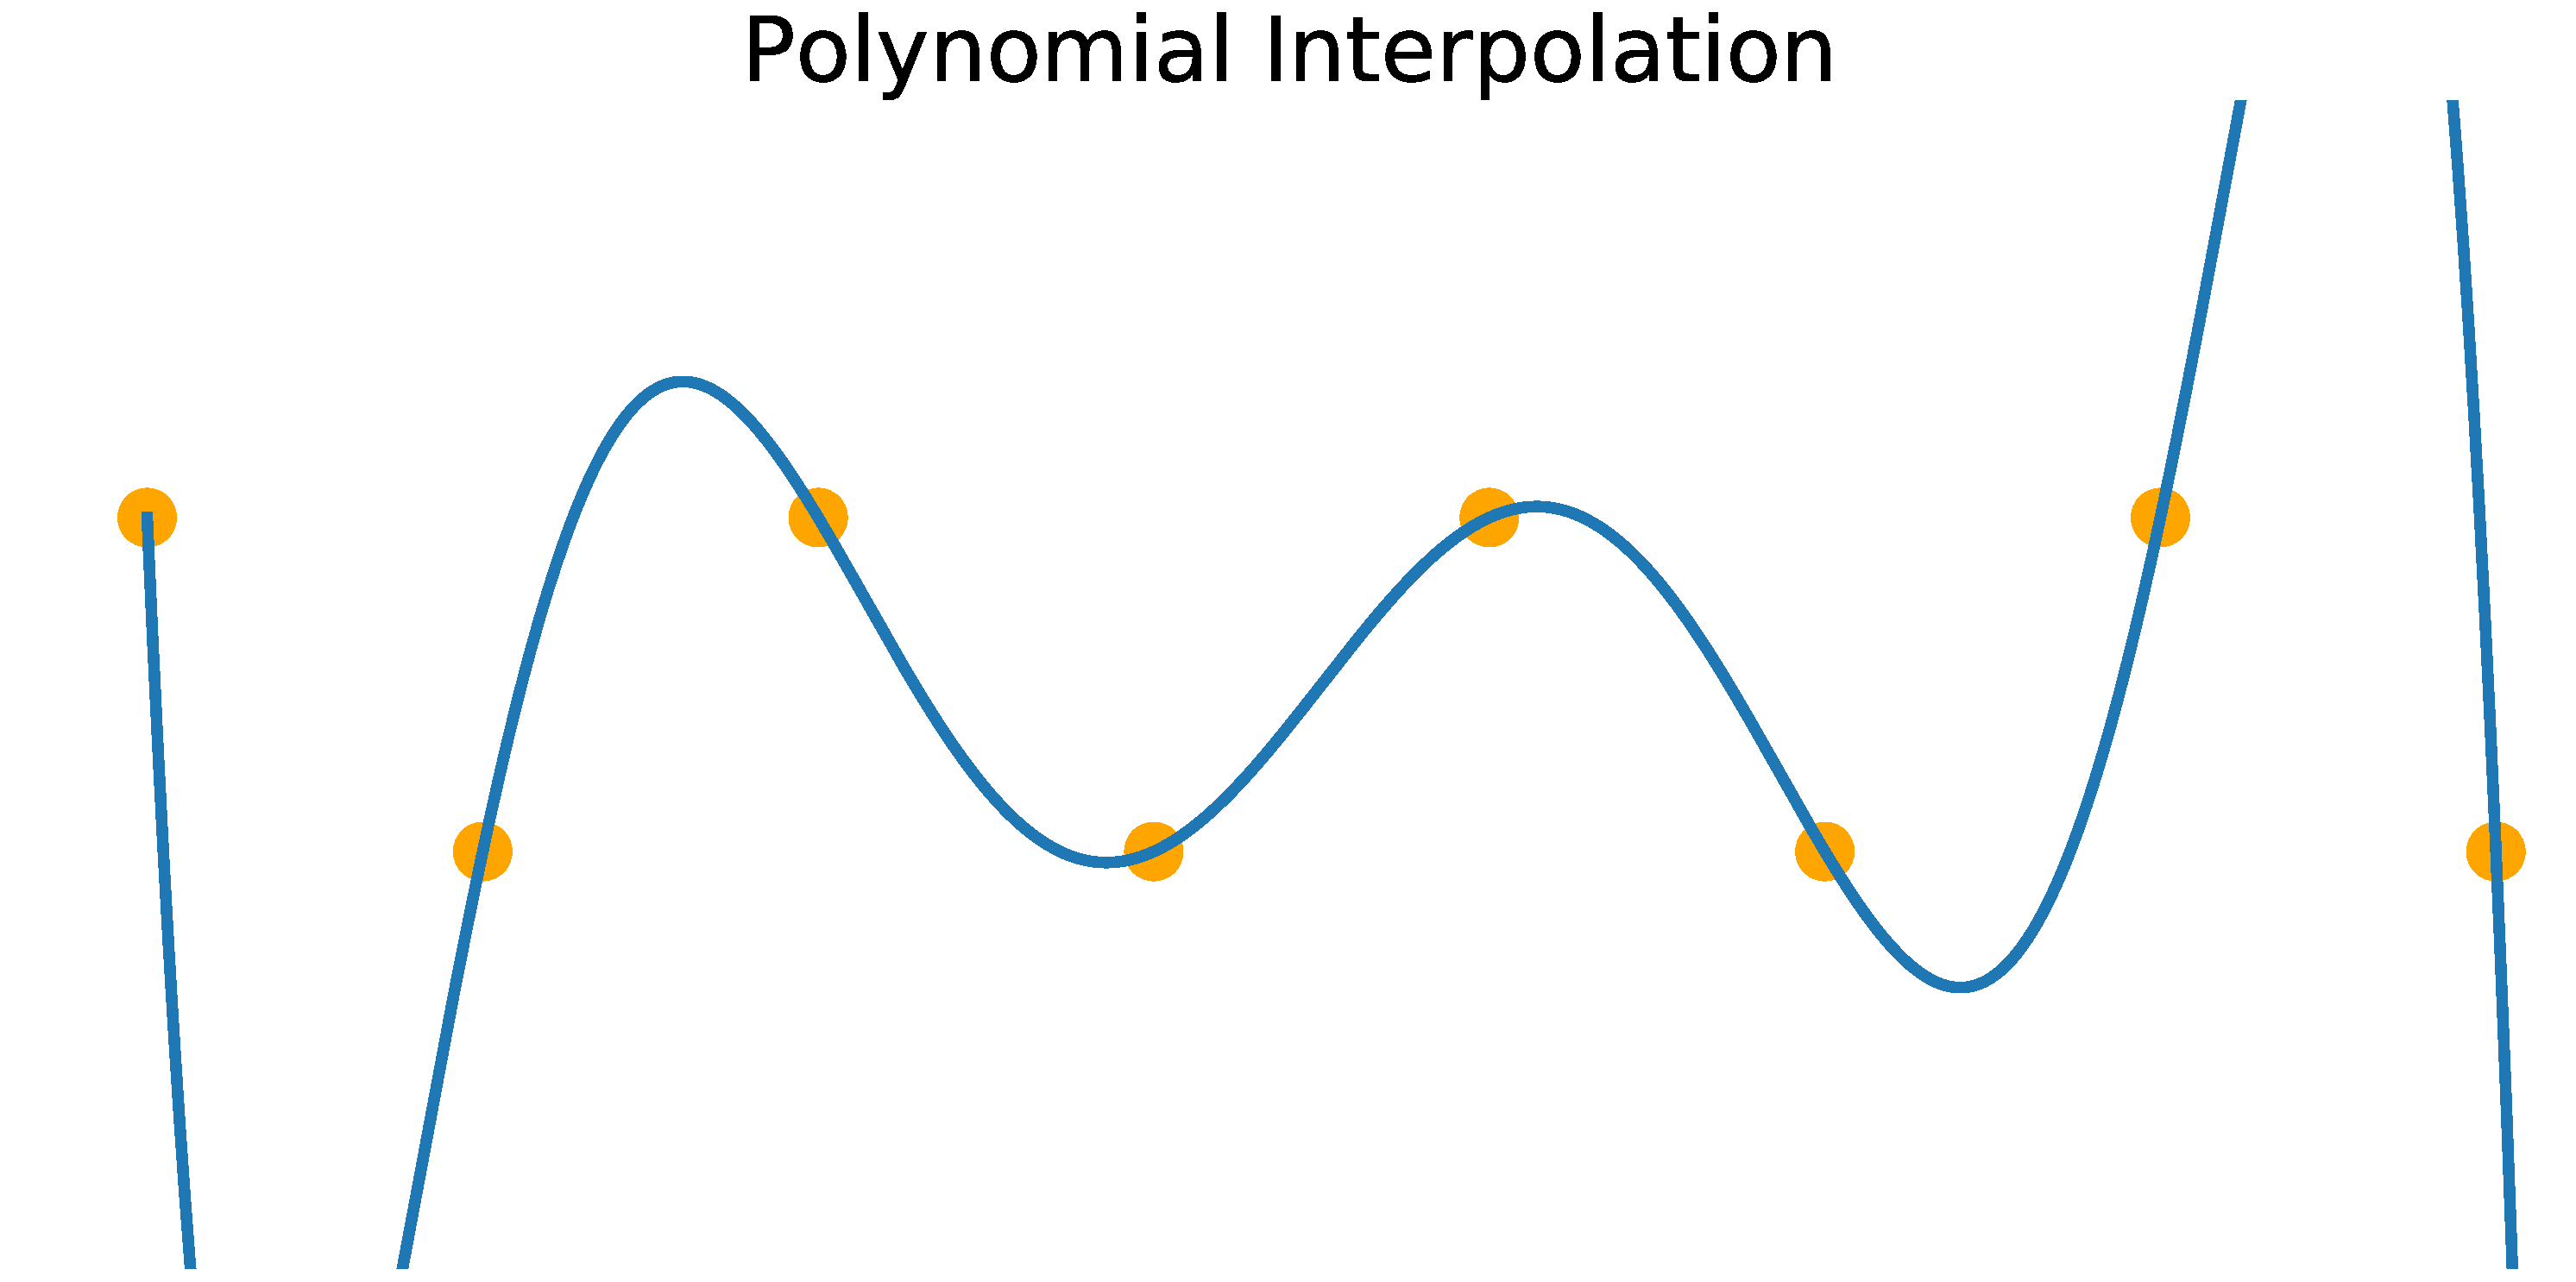
\includegraphics[width=.8\textwidth]{figures/poly_interp}
\end{figure}

Because the potential degree of the interpolated polynomial grows with the number of samples, polynomial interpolation can become very unstable when used on more than a few samples.

\textbf{Sinc Interpolation} \\
Last but not least, sinc interpolation lets us recover the original signal from samples exactly. However, we require that we sample the signal at with a sampling frequency greater than twice the highest frequency in the original signal. This property is known as the \textbf{Nyquist-Shannon Sampling Theorem}, which we will explore more in the next section.
\newline
Sinc interpolation relies on the $\mathrm{sinc}$ function, defined below.
\begin{equation*}
\mathrm{sinc}(t) = \begin{cases}
1 & t = 0 \\
\frac{\sin{} (\pi t)}{\pi t} & t \neq 0 \\
\end{cases}
\end{equation*}

\begin{figure}[H]
\centering
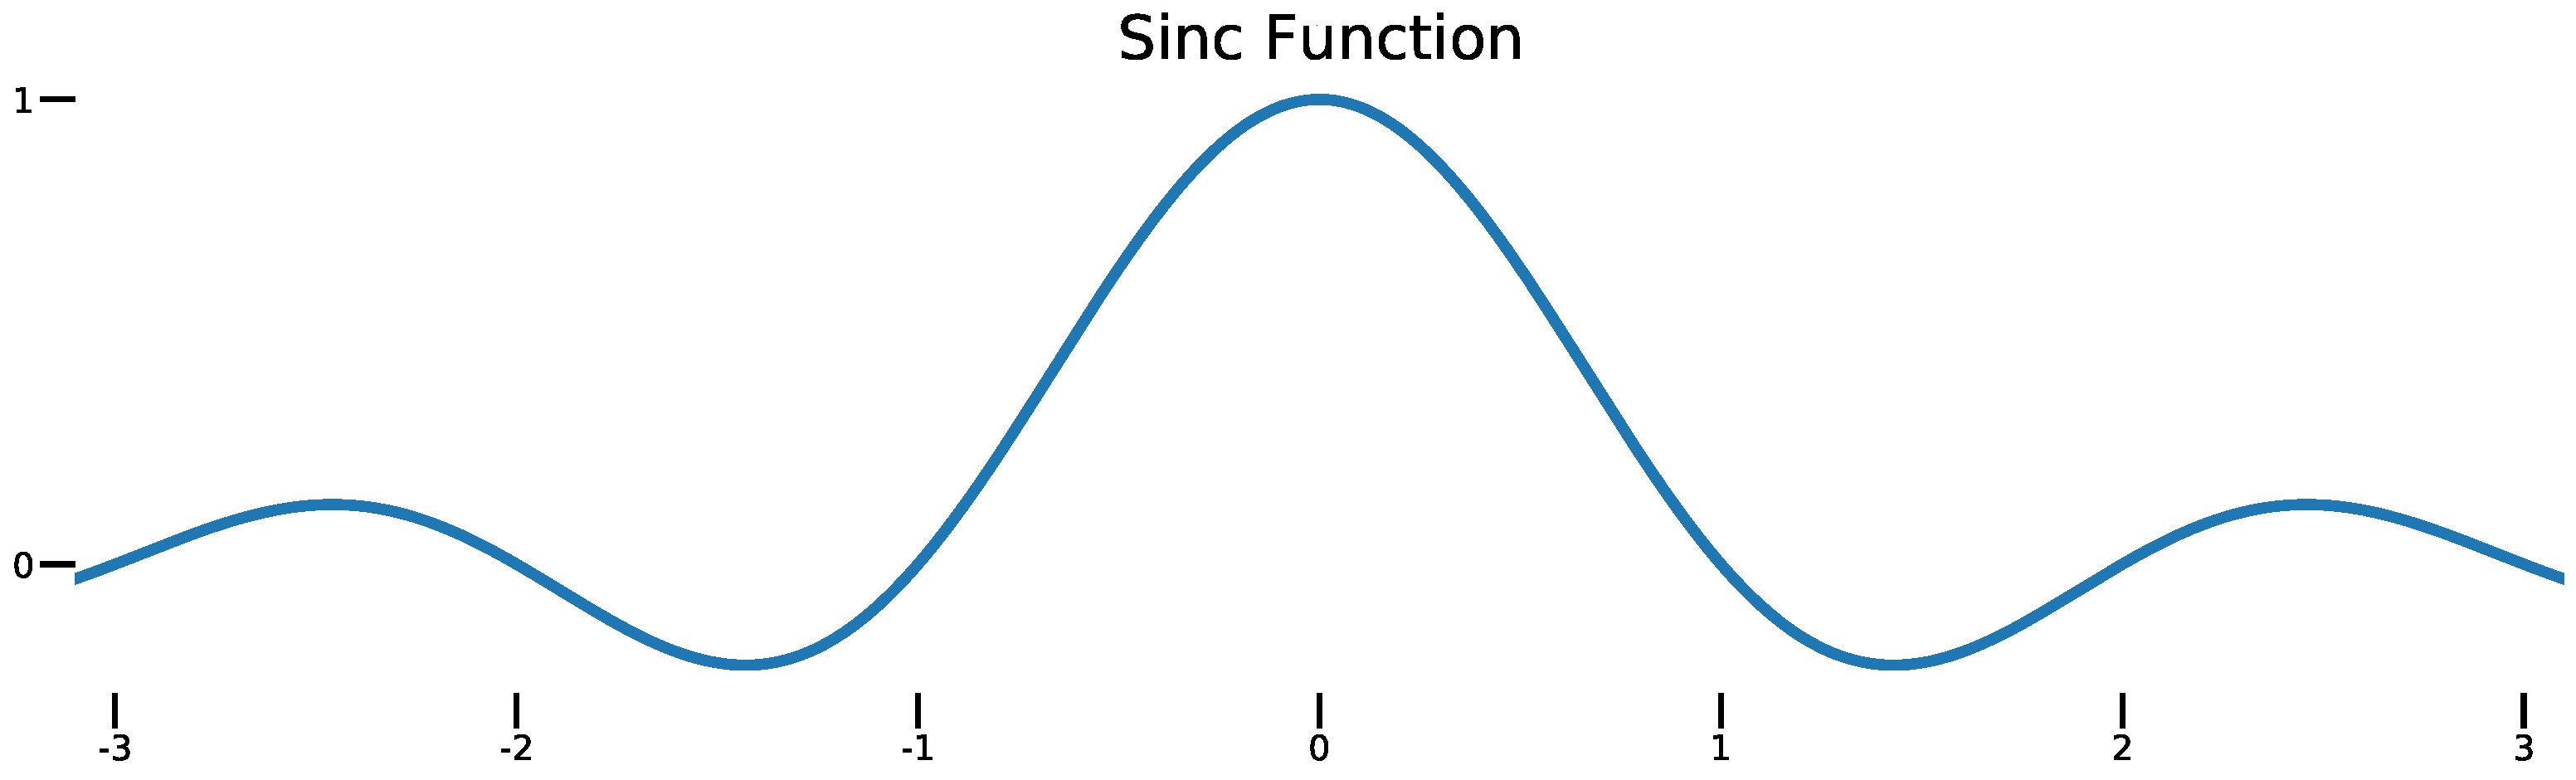
\includegraphics[width=.8\textwidth]{figures/sinc}
\end{figure}

However, we need to modify the signal a bit before we can use it as a basis function. We need to make sure that this signal takes on the value zero at every sample point, so we define the basis function as
\begin{equation*}
    \phi(t) = \mathrm{sinc}(\frac{t}{\Delta})
\end{equation*}

\begin{figure}[H]
\centering
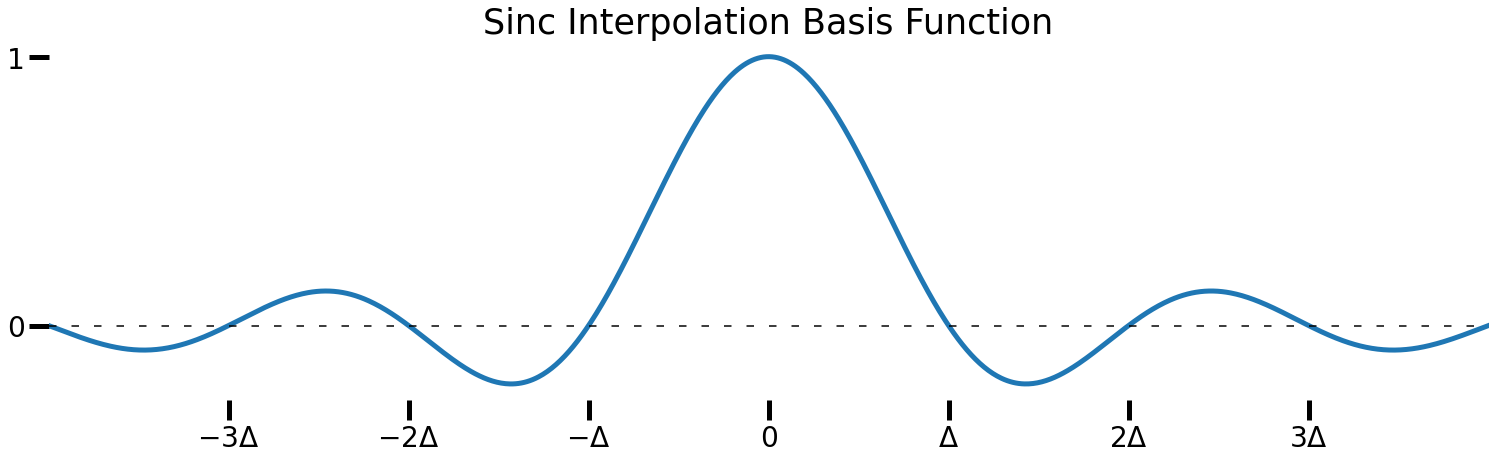
\includegraphics[width=.8\textwidth]{figures/sinc_basis}
\end{figure}

The resulting interpolation is
\begin{figure}[H]
    \begin{tikzpicture}
        \node (left) {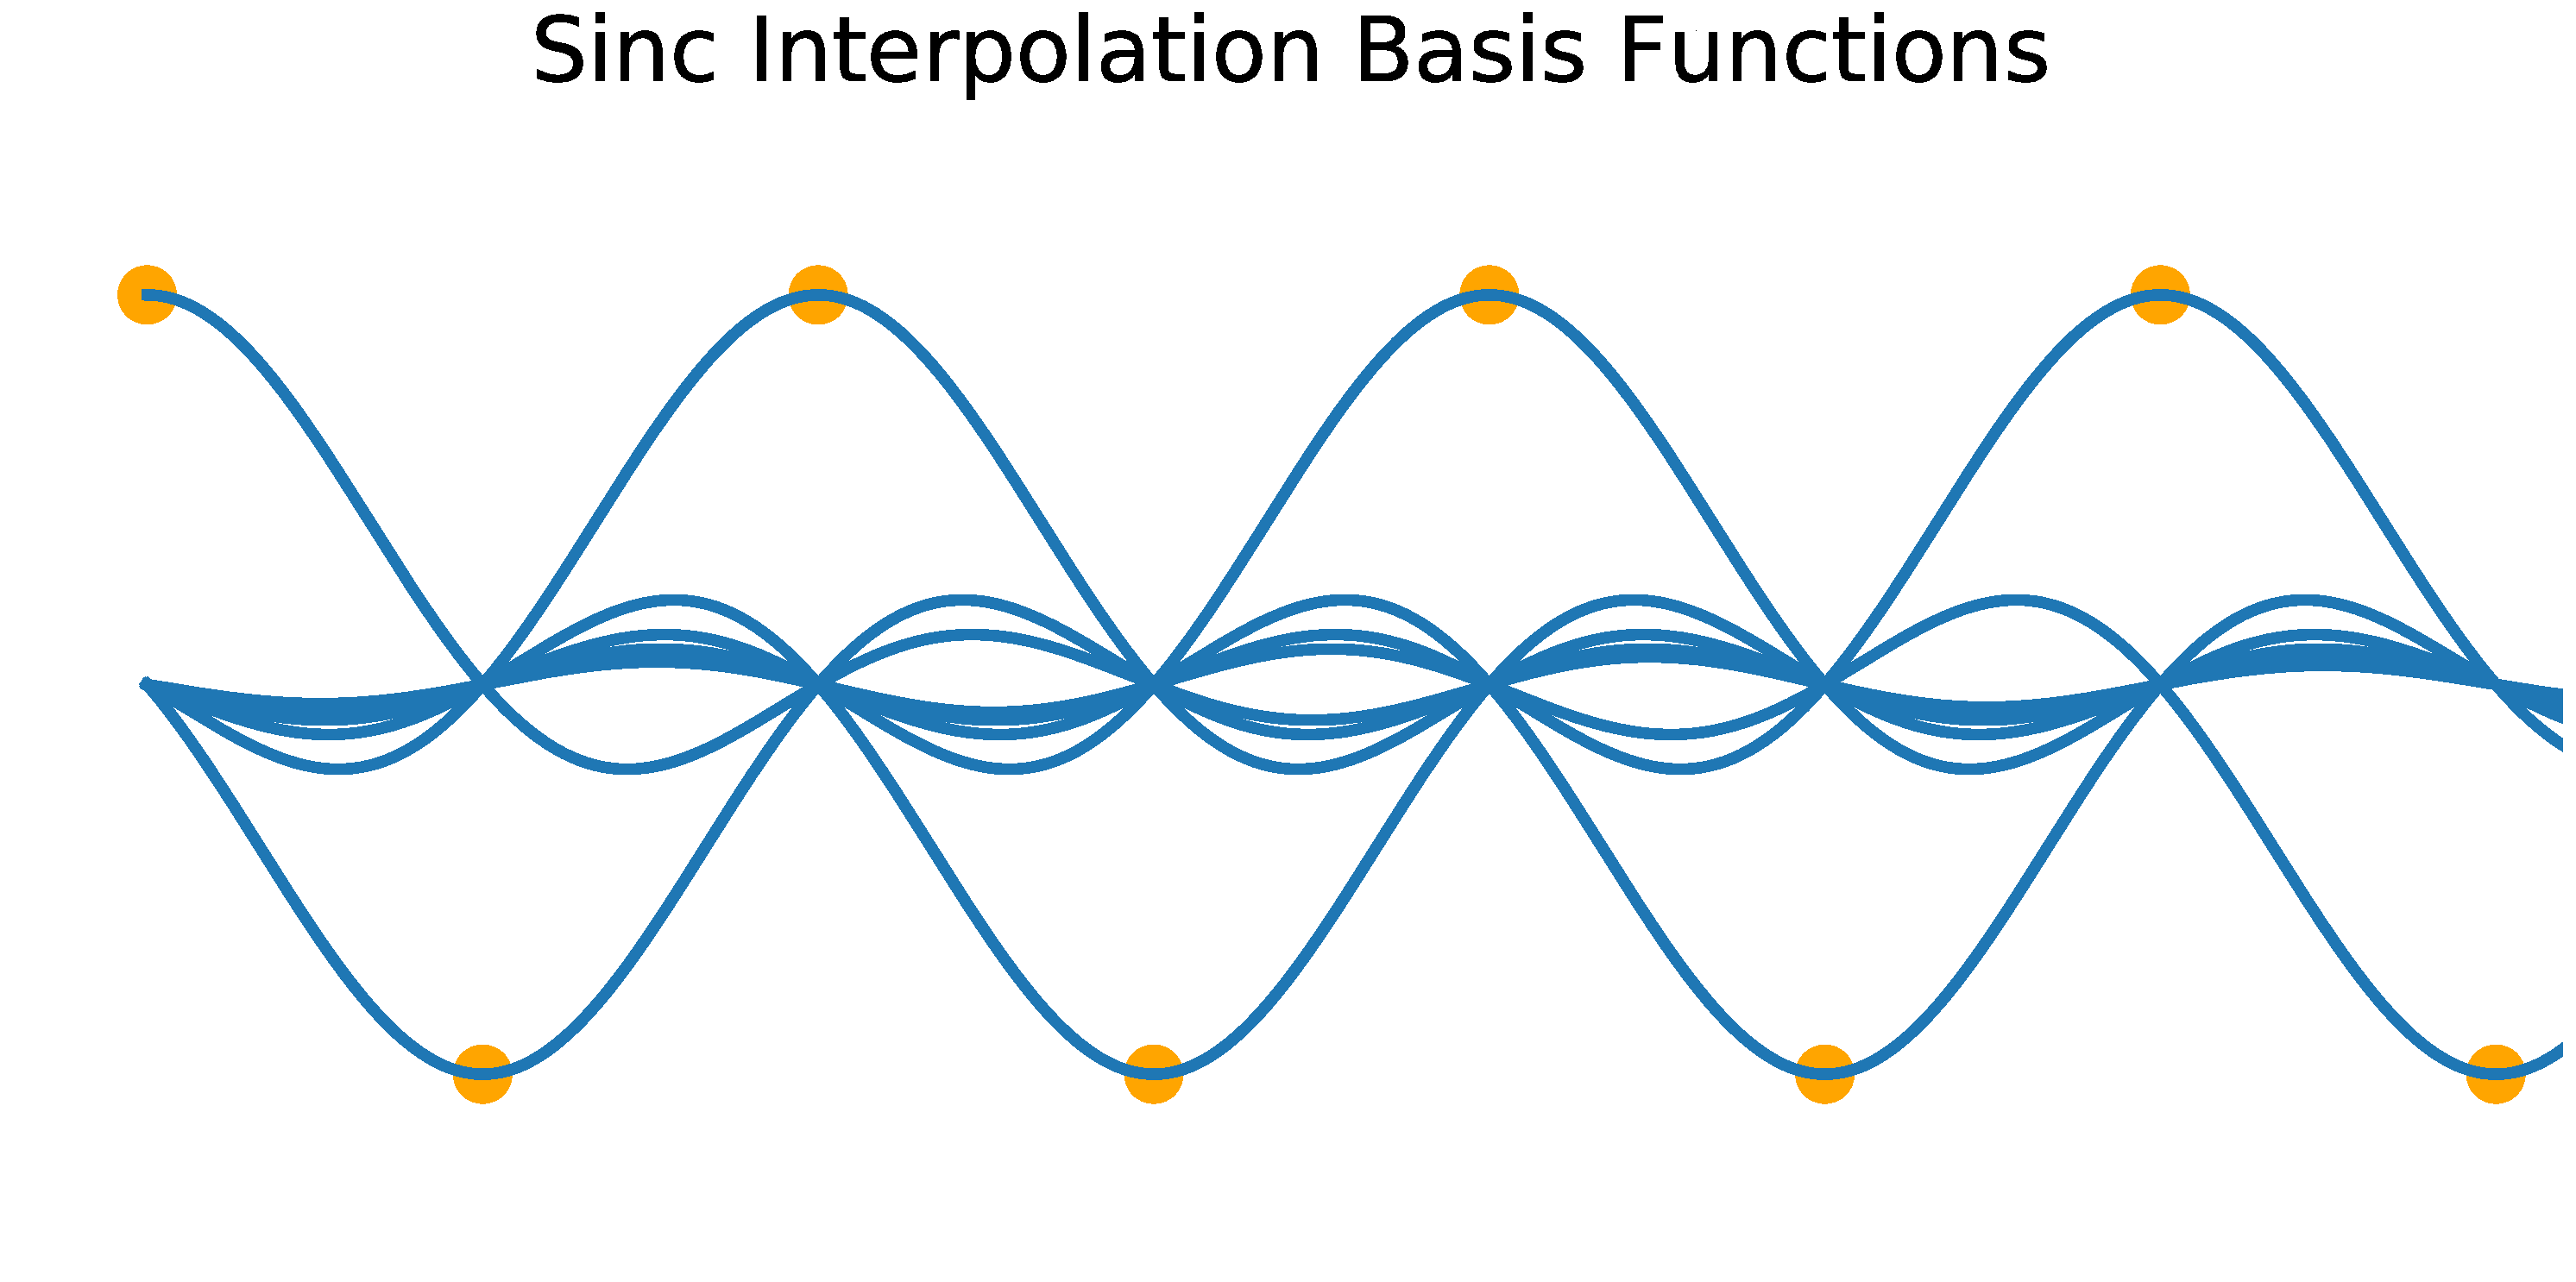
\includegraphics[width=8cm]{figures/sinc_interp_basis}};
        \node (right) [right=of left] {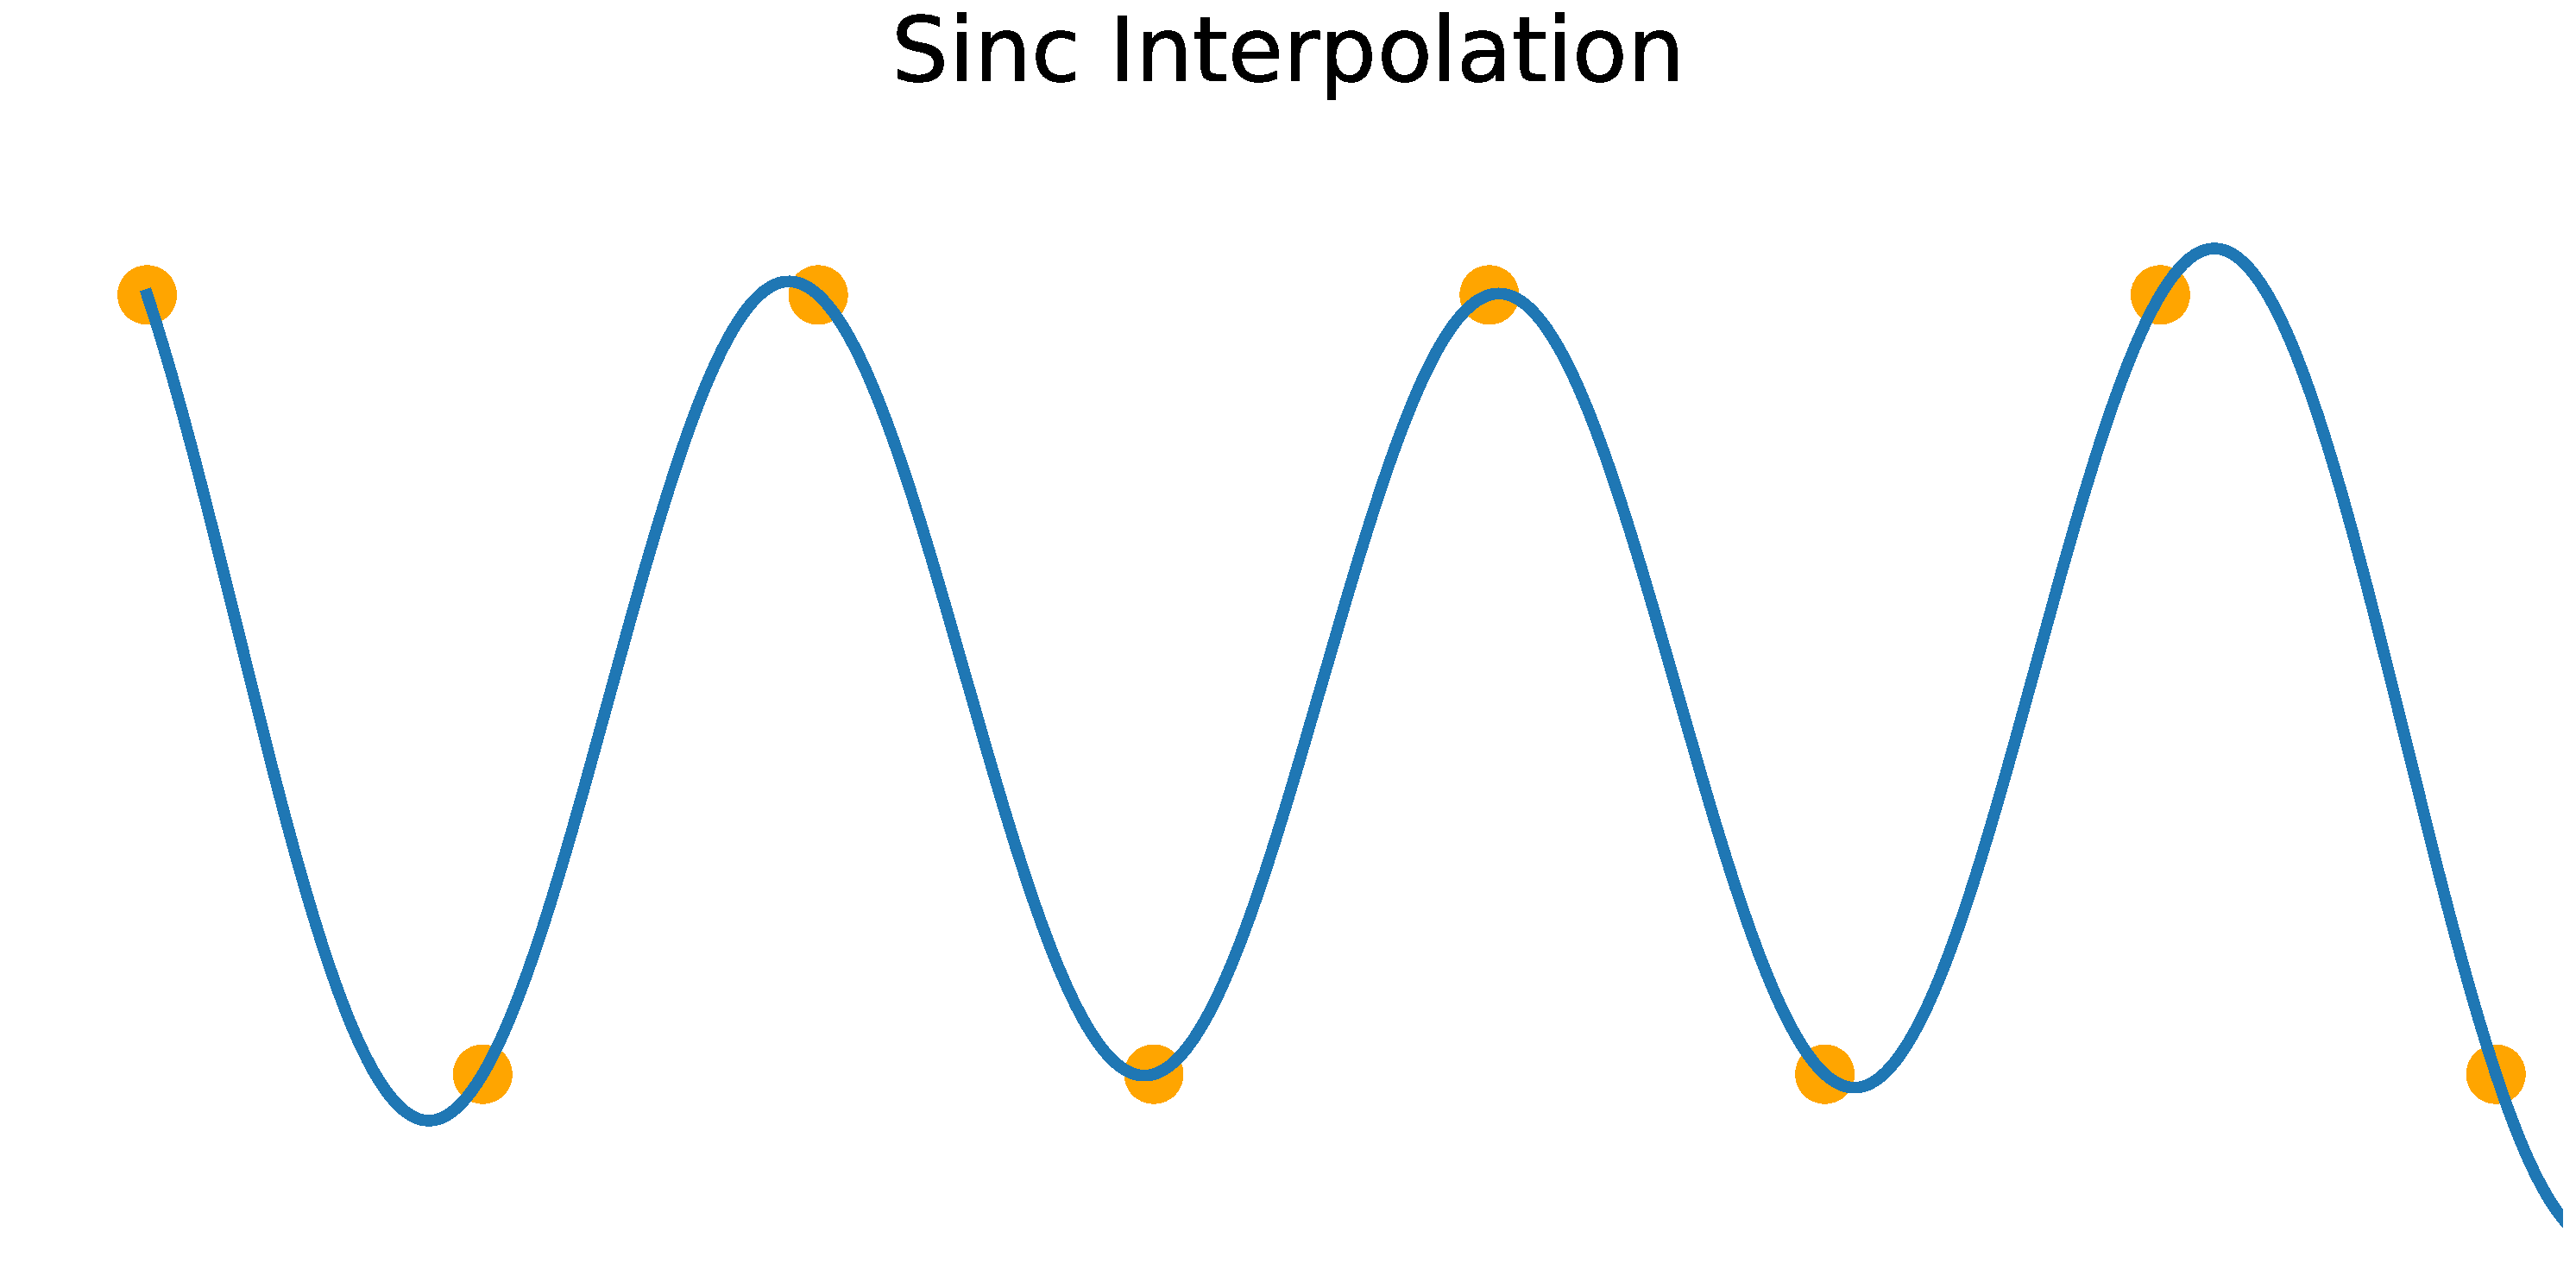
\includegraphics[width=8cm]{figures/sinc_interp}};
        \path[->] [line width = .5mm] (left) edge (right);
    \end{tikzpicture}
\end{figure}



\textbf{Nyquist Sampling Theorem and Aliasing} \\




\end{document}
